\documentclass[12pt]{article}
\usepackage[english]{babel}
\usepackage{natbib}
\usepackage{url}
\usepackage[utf8x]{inputenc}
\usepackage{amsmath}
\usepackage{graphicx}
\usepackage{hyperref}
\graphicspath{{images/}}
\usepackage{parskip}
\usepackage{float}
\usepackage{fancyhdr}
\usepackage{lastpage}
\usepackage{subcaption}
\usepackage[export]{adjustbox}
%\usepackage[bottom]{footmisc}
\usepackage[stable]{footmisc}
\usepackage{tikz}
\usepackage{tabularx}
\usetikzlibrary{shapes.geometric,arrows} 
\newcommand{\subsubsubsection}[1]{\paragraph{#1}\mbox{}\\}
\setcounter{secnumdepth}{4}
\setcounter{tocdepth}{4}
\usepackage{hyperref}

\hypersetup{
    colorlinks=true,
    linkcolor=blue,
    filecolor=cyan,      
    urlcolor=magenta,
}

\urlstyle{same}

%\usepackage{vmargin}
%\setmarginsrb{2 cm}{2.5 cm}{3 cm}{2.5 cm}{1 cm}{1.5 cm}{1 cm}{1.5 cm}

\topmargin=-0.5in    
\textheight=9in     %24.1cm
\evensidemargin=0in %0cm
\oddsidemargin=0in  %-.3cm
\textwidth=6.5in    %16.5cm

\title{Assignment: Group 10 \\ on \\ \vspace{0.5cm} Numerical solutions to porous fins}								% Title
\author{R Surya Narayan \\ Rino Raj P \\Ritesh Kumar Singh \\ Satyesh Raj }								% Author
\date{\today}											% Date

\makeatletter
\let\thetitle\@title
\let\theauthor\@author
\let\thedate\@date
\makeatother

\pagestyle{fancy}
\fancyhf{}
\rhead{Group 10}
\lhead{Computational Fluid Dynamics}
\cfoot{\thepage}

\begin{document}
\vspace{-2cm}
%%%%%%%%%%%%%%%%%%%%%%%%%%%%%%%%%%%%%%%%%%%%%%%%%%%%%%%%%%%%%%%%%%%%%%%%%%%%%%%%%%%%%%%%%

\begin{titlepage}
	\centering
    %\vspace*{0.1 cm}
    \textsc{\LARGE National Institute of Technology \\ \vspace{0.5cm} Tiruchirappalli}\\[1.5 cm]	% University Name
    
\includegraphics[scale = 0.2]{nitt_logo.png}\\[1.0 cm]	% University Logo
	\textsc{\Large CFD MEPE11}\\[0.5 cm]				% Course Code
	\textsc{\large Computational Fluid Dynamics}\\[0.5 cm]				% Course Name
	\rule{\linewidth}{0.2 mm} \\[0.4 cm]
	{ \huge \bfseries \thetitle}\\
	\rule{\linewidth}{0.2 mm} \\[1.5 cm]
	
    {\large \thedate}\\[1 cm]
    
	\begin{minipage}{0.4\textwidth}
		\begin{flushleft} \large
			\emph{Authors:}\\
			\theauthor
			\end{flushleft}
			\end{minipage}~
			\begin{minipage}{0.4\textwidth}
			\begin{flushright} \large
			\emph{Student ID:} \\
			111118091 \\ 211320021 \\ 211320022 \\ 111118095% Your Student Number
		\end{flushright}
	\end{minipage}\\
	
	
 
	\vfill
	
\end{titlepage}

%%%%%%%%%%%%%%%%%%%%%%%%%%%%%%%%%%%%%%%%%%%%%%%%%%%%%%%%%%%%%%%%%%%%%%%%%%%%%%%%%%%%%%%%%

{\small \tableofcontents}
\pagebreak

\flushbottom

%%%%%%%%%%%%%%%%%%%%%%%%%%%%%%%%%%%%%%%%%%%%%%%%%%%%%%%%%%%%%%%%%%%%%%%%%%%%%%%%%%%%%%%%%

\section{Introduction and Motivation}
\subsection{On fins}
Fins basically are protrusions or extended surfaces on the outer surface of equipment that require heat transfer between themselves and their immediate surroundings. Typically these are used to dissipate heat to the surroundings faster, as they enhance the heat transfer rates by providing extra surface area. However the placing of extra surfaces to enhance heat transfer can also decrease the mean temperature at which the surface looses heat to the surroundings, as the fin itself possesses finite non-zero conductivity $k$, resulting in a decrease of temperature (from the base temperature $T_{base}$) along the fin length. Hence fin-design requires careful considerations between the internal gradients set-up along the fin-length to the net surface area we increase for heat transfer. These can be quantitatively characterized using the \emph{efficiency} and the \emph{effectiveness}. While the former reflects the performance of the fin relative to one with infinite conductivity, the latter examines the improvement/reduction in heat-transfer due to its very presence. Fins have been used extensively to dissipate heat from hot surfaces. Typical applications of \emph{cooling fins} include:
\begin{itemize}
    \item air-cooled two-stroke engines of motorcycles
    \item electronic cooling applications like CPU and GPU cooling,
    \item compressors and their inter-coolers (for multi-stage compressors)  
    \item radiators of cars
\end{itemize}
Heating fins are relatively sparse in terms of application however a few examples exist. One may use fins, for instance, in the surface of heat exchanger pipes to  enhance heat transfer. Increasing fin performance has been a subject of intensive research and porous fins have shown to be very promising in the paper given to our group. 
\subsection{On the general physics of the problem}
The paper given to was titled \emph{``Thermal analysis of porous pin fin used for electronic cooling"}. This paper derives the entire analytical framework required for extending a simple fin analysis to a \emph{porous fin} analysis. This section is dedicated to examining some heuristics of the problem that can follow from basic principles of physics. This can help make some common sense judgements of the results we obtain and judge the correctness of the trends obtained in graphs between various quantities. The basic aspects of fins and their physics is already presented in brief in the section 1.1.\\ \\
With the introduction of pores in the fin, there is greater surface area exposed for heat transfer hence the expectation is that they must perform better. However, one must also keep in mind the decrease in the overall thermal conductivity of the fin because of the presence of pores. While previously the pores had high-conductivity fin material, they are now replaced with air or the surrounding medium whose flow is now subject to natural convection. The thermal conductivity of the fluid is much less in comparison with the fin material hence lowering the mean surface temperature of heat loss. Hence one can observe two opposing effects at play. However, it is found from theoretical studies in the paper, that the area increase outweighs the reduced heat transfer due to a decrease in the effective thermal conductivity. Natural convection through the pores dominates over the poor conductivity of the fluid, hence augmentation in fin performance is much higher for the porous fin when there are improvements made to the convective heat transfer coefficient $h$. The Rayleigh number, $Ra$ is a good indicator of the amount of natural convection. Hence it follows that an increase in the $Ra$ number must result in increased heat transfer rate and performance. Since the interaction between the fluid and the fin is \emph{volumetric}, i.e. affected in 3-D space because of the pores dispersed throughout the volume, the increase in heat-transfer is much larger for an increase in $Ra$.  We now look at the associated changes in the mathematics and the governing differentiatial equation that arises due to the introduction of pores.
\subsection{On the Governing Differential Equation\footnote{shortened as GDE henceforth}}
The mathematics of a traditional extended surface or a fin is quite simple and can be derived by balancing the convective and convective heat transfer through a cross-section. The result is an easy to solve $2^{nd}$ order ODE given by:
\[
\frac{d^2\theta}{dx^2} = m^2 \theta \tag{1} \label{1}
\]
where $\theta$ and $m$ are parameters given by \eqref{2} and \eqref{3} to make the fin analysis as general as possible:
\[
\theta = T-T_\infty \tag{2} \label{2}
\]
\[
m = \sqrt{\frac{hP}{kA}} \tag{3} \label{3}
\]
When a porous fin is considered there should be some variable that accounts for how ``filled" or empty the fin is. This is represented by the parameter $\xi$ which is called the porosity or void ratio. After suitable introduction of the parameter $\xi$ (the math is skipped presently as it can be found in the paper) we get the following modified equation in-terms of the basic parameters and the temperature $T$: 
\[
\frac{d^2T}{dx^2} - \frac{4\rho c_p gK\beta(T-T_a)^2}{\gamma D k_{eff}} - \frac{4h(1-\xi)(T-T_a)}{Dk_{eff}} = 0 \tag{4} \label{4}
\]
The above is obtained by considering the net convection loss due to the pores and equating it to the conductive heat flux using the Fourier's law of heat conduction. To retain generality of analysis the above equation is non-dimensionalized. The spatial and physical properties are non-dimensionalized as: 
\[
(X,\psi,k_r,\theta) = \left(\frac{x}{L}, \frac{R}{L}, \frac{k_s}{k_f}, \frac{T-T_a}{T_b-T_a}\right) \tag{5} \label{5}
\]
The non-dimensional numbers that naturally hence arise are:
\[
(Nu, Ra, Da) = \left(\frac{hD}{k_f}, \frac{\rho c_p g \beta D^3 (T_b-T_a)}{\gamma k_f}, \frac{K}{D^2}\right) \tag{6} \label{6}
\]
The effects of these numbers are naturally wrapped up as coefficients in the parent GDE as:
\[
(\omega_1, \omega_2) = \left(\frac{Ra Da}{\Omega \psi^2}, \frac{Nu(1-\xi)}{\Omega \psi^2}\right) \tag{7} \label{7}
\]
where $\Omega$ denotes the dimensionless effective conductivity:
\[
\Omega = \xi + (1-\xi)k_r \tag{8} \label{8}
\]
The parent GDE that becomes the main consideration for this assignment hence becomes: 
\[
\frac{d^2\theta}{dX^2} = \omega_1 \theta + \omega_2 \theta \tag{9} \label{9}
\]
This report focuses on seeking solutions to \eqref{9}, which is a \emph{non-linear $2nd$ order ODE}. Analytical solutions to the ODE \eqref{9} are not readily possible. Further details on analytical and semi-analytical solutions to the equation can be found in \hyperref[sec:analytical]{section 2}.

\subsection{On the Boundary Conditions for fin problems}
Boundary conditions to solve \eqref{1} are dictated by the physics of the problem and depend on the way we intend to model the fin. Since the ODE is second order we would require two BCs. However one boundary condition common to all types is the Dirichlet boundary condition at the base:
\[
\theta(x=0) = \theta_{base} = T_{base} - T_\infty \tag{10} \label{10}
\]
The second BC is at the other end of the fin and depends on the type of modelling and we would apply to it. For a fixed temperature at the other end, it would simply be a Dirichlet BC:
\[
\theta (x= L) = \theta_L = T_{L} - T_\infty \tag{11} \label{11}
\]
For fins that convect zero heat to the surroundings at the tip, the BC becomes a Neumann BC: 
\[
\frac{d\theta}{dx}\Bigr|_{x=L} = 0 \tag{12} \label{12}
\]
A third possible scenario is when there is a Robin BC (or a mixed BC) in the end, i.e. the heat loss from convection is finite: 
\[
h\theta_L = -k\frac{d\theta}{dx}\Bigr|_{x=L} \tag{13} \label{13}
\]
A fourth possible case is the assumption that the fin is extremely long, i.e. $L\to\infty$ resulting in \[
\theta (x=L) = T_L-T_\infty = 0 \tag{14} \label{14}  
\]
For the parent GDE represented by \eqref{8} we impose a Neumann BC at $X=0$ and a Dirichlet BC at $X=1$.
\[
\theta (X=1) = 1 \tag{15} \label{15}
\]
\[
\frac{d\theta}{dx}\Bigr|_{X=0} = 0 \tag{16} \label{16}
\]
Note that we start $X=0$ at the tip of the fin as presented in figure \ref{fig:1}
\begin{figure}
    \centering
    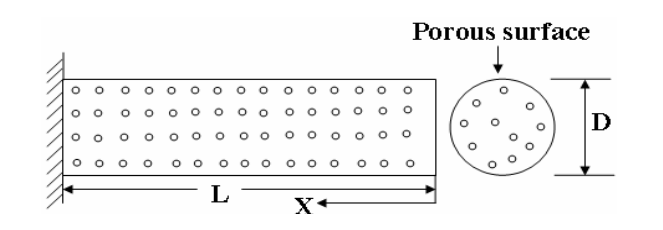
\includegraphics[scale=1]{Description/prob.PNG}
    \caption{Physical representation of the problem}
    \label{fig:1}
\end{figure}
\section{Analytical Solutions}\label{sec:analytical}
\subsection{The ODE Problem and its difficulties}
This section expands on the analytical solution to the ODE problem we are interested in. For the sake of clarity we restate the ODE problem we are tasked with solving (\eqref{9}, \eqref{15} and \eqref{16}):
\[  
\frac{d^2\theta}{dX^2} = \omega_1 \theta + \omega_2 \theta \tag{9} 
\]
With the boundary conditions:
\[
\theta (X=1) = 1 \tag{15} 
\]
\[
\frac{d\theta}{dx}\Bigr|_{X=0} = 0 \tag{16} 
\]
The above ODE problem as mentioned previously is a $2^{nd}$ non-linear ODE that belongs to the general class of autonomous ODE problems represented by:
\[
\frac{d^2y}{dx^2} = f(y) \tag{17} \label{17}
\]
\href{http://eqworld.ipmnet.ru/en/solutions/ode/ode0301.pdf}{This reference} suggests the general solution to such a class of problems is: 
\[
\int \left(C_1 + 2\int f(y)dy\right)^{-\frac{1}{2}}dy = C_2 \pm x \tag{18} \label{18}
\]
In our case:
\[
f(y) = \omega_1 y + \omega_2 y^2 \tag{19} \label{19}
\]
However the resulting integral after substitution into the mentioned formula assumes the form: 
\[
C_2 \pm x = \int \frac{1}{\sqrt{Ay^3 + By^2 + C}} dy \tag{20} \label{20} 
\]
which becomes very complicated to solve. Hence the need for numerical or a semi-analytical solution to the ODE is felt.
\subsection{Adomain Decomposition}
The authors present a new semi-analytical approach to the above ODE in their paper using a new method based on adomain decomposition. The reader is referred to the paper for the details of its derivation. Broadly speaking, the method seeks to approximate the solution using a series of polynomials by using the second-differential $\frac{d^2}{dX^2}$ as an invertible operator. The final solution the ODE problem represented by \eqref{9} using adomain decomposition is simplified and finally presented here from the said reference: 
\[
\theta = \theta_0 + P_1(\omega_1,\omega_2, \theta_0) X^2 + 
                    P_2(\omega_1,\omega_2, \theta_0) X^4 +
                    P_3(\omega_1,\omega_2, \theta_0) X^6 +
                    P_4(\omega_1,\omega_2, \theta_0) X^8+ ..  \tag{21} \label{21}
\]
Where $\theta_0$ represents the dimensionless temperature at $X=0$ and needs to be found out by solving the transcendental algebraic equation given by \eqref{22}. This follows directly by substituting the boundary conditions on the equation \eqref{21}.  
\[
1 - \theta_0  - P_1(\omega_1,\omega_2, \theta_0) X^2 - 
                    P_2(\omega_1,\omega_2, \theta_0) X^4 -
                    P_3(\omega_1,\omega_2, \theta_0) X^6 -
                    P_4(\omega_1,\omega_2, \theta_0) X^8+ .. = 0  \tag{22} \label{22}
\]
$P_1$, $P_2$, $P_3$ and $P_4$ here are polynomials given by equations \eqref{23}, \eqref{24}, \eqref{25} and \eqref{26}: 
\[
P_1(\omega_1,\omega_2,\theta_0) = (\omega_1 \theta_0^2 + \omega_2 \theta_0) \frac{1}{2!} \tag{23} \label{23}
\]
\[
P_2(\omega_1,\omega_2,\theta_0) = (2 \omega_1^2 \theta_0^3 + 3\omega_1 \omega_2 \theta_0^2 + \omega_2^2 \theta_0)\frac{1}{4!} \tag{24} \label{24}
\]
\[
P_3(\omega_1,\omega_2,\theta_0) = (10 \omega_1^3 \theta_0^4 + 20 \omega_1^2\omega_2 \theta_0^3 + 11 \omega_1 \omega_2 \theta_0^2 + \omega_2^3 \theta_0)\frac{1}{6!} \tag{25} \label{25}
\]
\[
P_4(\omega_1,\omega_2,\theta_0) = (80 \omega_1^4 \theta_0^5 + 200 \omega_1^3 \omega_2 \theta_0^4 + 162 \omega_1^2 \omega_2^2 \theta_0^3 + 43 \omega_1 \omega_2^3 \theta_0^2 + \omega_2^4 \theta_0)\frac{1}{8!}\tag{26} \label{26}
\]
Hence to find the analytical solution one needs to first solve for the variable $\theta_0$ using \eqref{22} and then substitute the values the polynomials take in \eqref{21}. Note that this technique isn't entirely analytical in itself as solutions to the highly non-linear equation \eqref{22} can only be obtained from numerical methods. Hence this can be called a semi-analytical and semi-numerical approach. The above solution is still isn't exact, as we have used only 4 polynomials to approximate the solution. One can use more polynomials for greater accuracy and closeness. Therefore this method itself carries a certain amount of error with itself and hence cannot be fully relied on. The subsequent sections elaborate on the implementation we followed to obtain the analytical solution using the approach outlined so far. 
\subsection{Algorithm }
The final algorithm we followed for obtaining the analytical solution is as follows:
\begin{enumerate}
    \item Input parameters specified in \eqref{7}
    \item Compute $\omega_1$ and $\omega_2$ using inputs of the previous step
    \item Compute $\theta_0$ using MATLAB \emph{fsolve} function and \eqref{22}
    \item Compute $P_1$, $P_2$, $P_3$ and $P_4$ using \eqref{23}, \eqref{24}, \eqref{25} and \eqref{26} respectively
    \item Generate $X_i$'s corresponding to the intended mesh
    \item Use \eqref{21} to compute $\theta_i$'s at the $X_i$'s 
    \item Plot results
\end{enumerate}
The MATLAB \emph{fsolve} function takes input arguments as a function and the initial guess to compute solutions to any non-linear equation represented by the argument function. 
\subsection{Implementation details}
This section deals with the implementation of the analytical solution to the problem thus presented. More on the development of the code, its organization and usage can be found in the \hyperref[sec:Code]{section 4}. We chose to go with MATLAB as the programming language due to its familiarity with all the team members and its user-friendliness. In-built plotting options enables immediate abd in-situ visualization of the solutions when obtained. In addition, MATLAB also houses several packages favourable to numerical computations like numerical solvers for ODEs, non-linear equations, optimization, linear solvers etc. A generic function named \href{https://rsuryanarayan.github.io/CFD_Documentation/}{``$analytical\_solution$"} was created with the mesh and the parameters in \eqref{7} as inputs. This enabled calling the function for any set of arguments and mesh size. Complete segmentation of the sub-functions and dependencies was done to make debugging and organization easy. The following figure gives the function call-graph (or a dependency graph) for the function thus mentioned:(click on ``Graphs" in the link to generate this)
\begin{figure}[H]
    \centering
    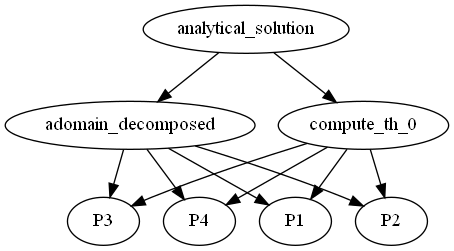
\includegraphics[scale=0.65]{Call graphs/callgraph_analytical.png}
    \caption{Call graph for the analytical solution}
    \label{fig:2}
\end{figure}
\subsection{Results}
This section presents the results of the MATLAB code developed by us to compute the analytical solution. The results largely depend on the accuracy to which \emph{fsolve} has solved the non-linear equataion \eqref{22}.To investigate this we obtained the first order optimality plot that describes the course of solution of the algorithm that \emph{fsolve} uses. First order optimality refers to the resuiduals of the objective function that \emph{fsolve} casts the parent non-linear problem into for finding gradient-search based solutions. To know more on the internal frameworks of \emph{fsolve} the reader is referred to the  \href{https://www.mathworks.com/help/optim/ug/fsolve.html#butbmfz-5}{documentation}. The algorithms used for optimization are \href{https://www.mathworks.com/help/optim/ug/equation-solving-algorithms.html#brnpdsm}{Trust-region}, \href{https://www.mathworks.com/help/optim/ug/equation-solving-algorithms.html#f51887}{Trust-region-Dogleg} and \href{https://www.mathworks.com/help/optim/ug/equation-solving-algorithms.html#f51887}{Levenberg-Marquadt} methods which are search-based optimization algorithms.   
\begin{figure}[h]
    \centering
    \includegraphics[scale=.8]{residual_plot_fsolve.png}
    \caption{First order optimality of \emph{fsolve}}
    \label{fig:3}
\end{figure}
The residuals of the first order optimality are obtained. For instance, the input paramter set $(Ra, Da, Nu, \xi, k_r) = (1000, 0.04, 10, 0.05, 0.8, 7000)$, the residuals drop to $7.59\times 10^{-7}$ (Figure \ref{fig:3}). Hence the solution to the non-linear equation \eqref{22} are satisfactory and accurate enough for all practical purposes. Using the computed $\theta_0$ we now compute the actual solution using the function \href{https://rsuryanarayan.github.io/CFD_Documentation/}{$``adomain\_decomposed"$}.The trends between $(X,\theta)$,$(\epsilon,\psi)$, $(\eta,\xi)$ and $(\epsilon,\xi)$. These graphs are presented in the next page. Upon comparison of the values at $X=0$ it is seen that the values are near the mark that the paper presents. However, this cannot be taken as a final confirmation of the results we have obtained. Further validation is required by solving it via numerical methods and comparing the analytical results with them. This shall serve as a validation both for the numerical and the analytical methods thus presented. The subsequent sections deal with the same. 
\begin{figure}[H]
\begin{minipage}{.5\textwidth}
    \hspace{-1.4cm}
    \vspace{-1.4cm}
  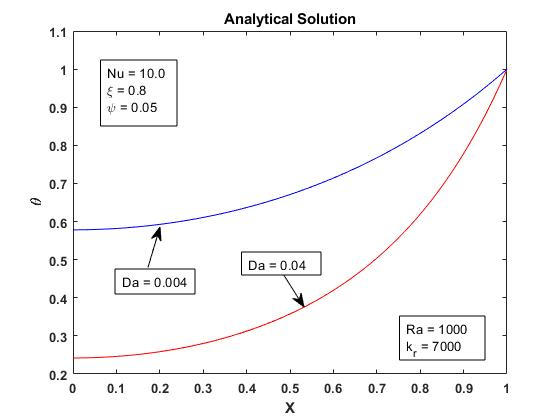
\includegraphics[scale=0.5]{Analytical Solution/Analytical graph.jpg}
  \label{fig:4}
\end{minipage}%
\begin{minipage}{.5\textwidth}
  \hspace{-0.5cm}
  \vspace{-1cm}
  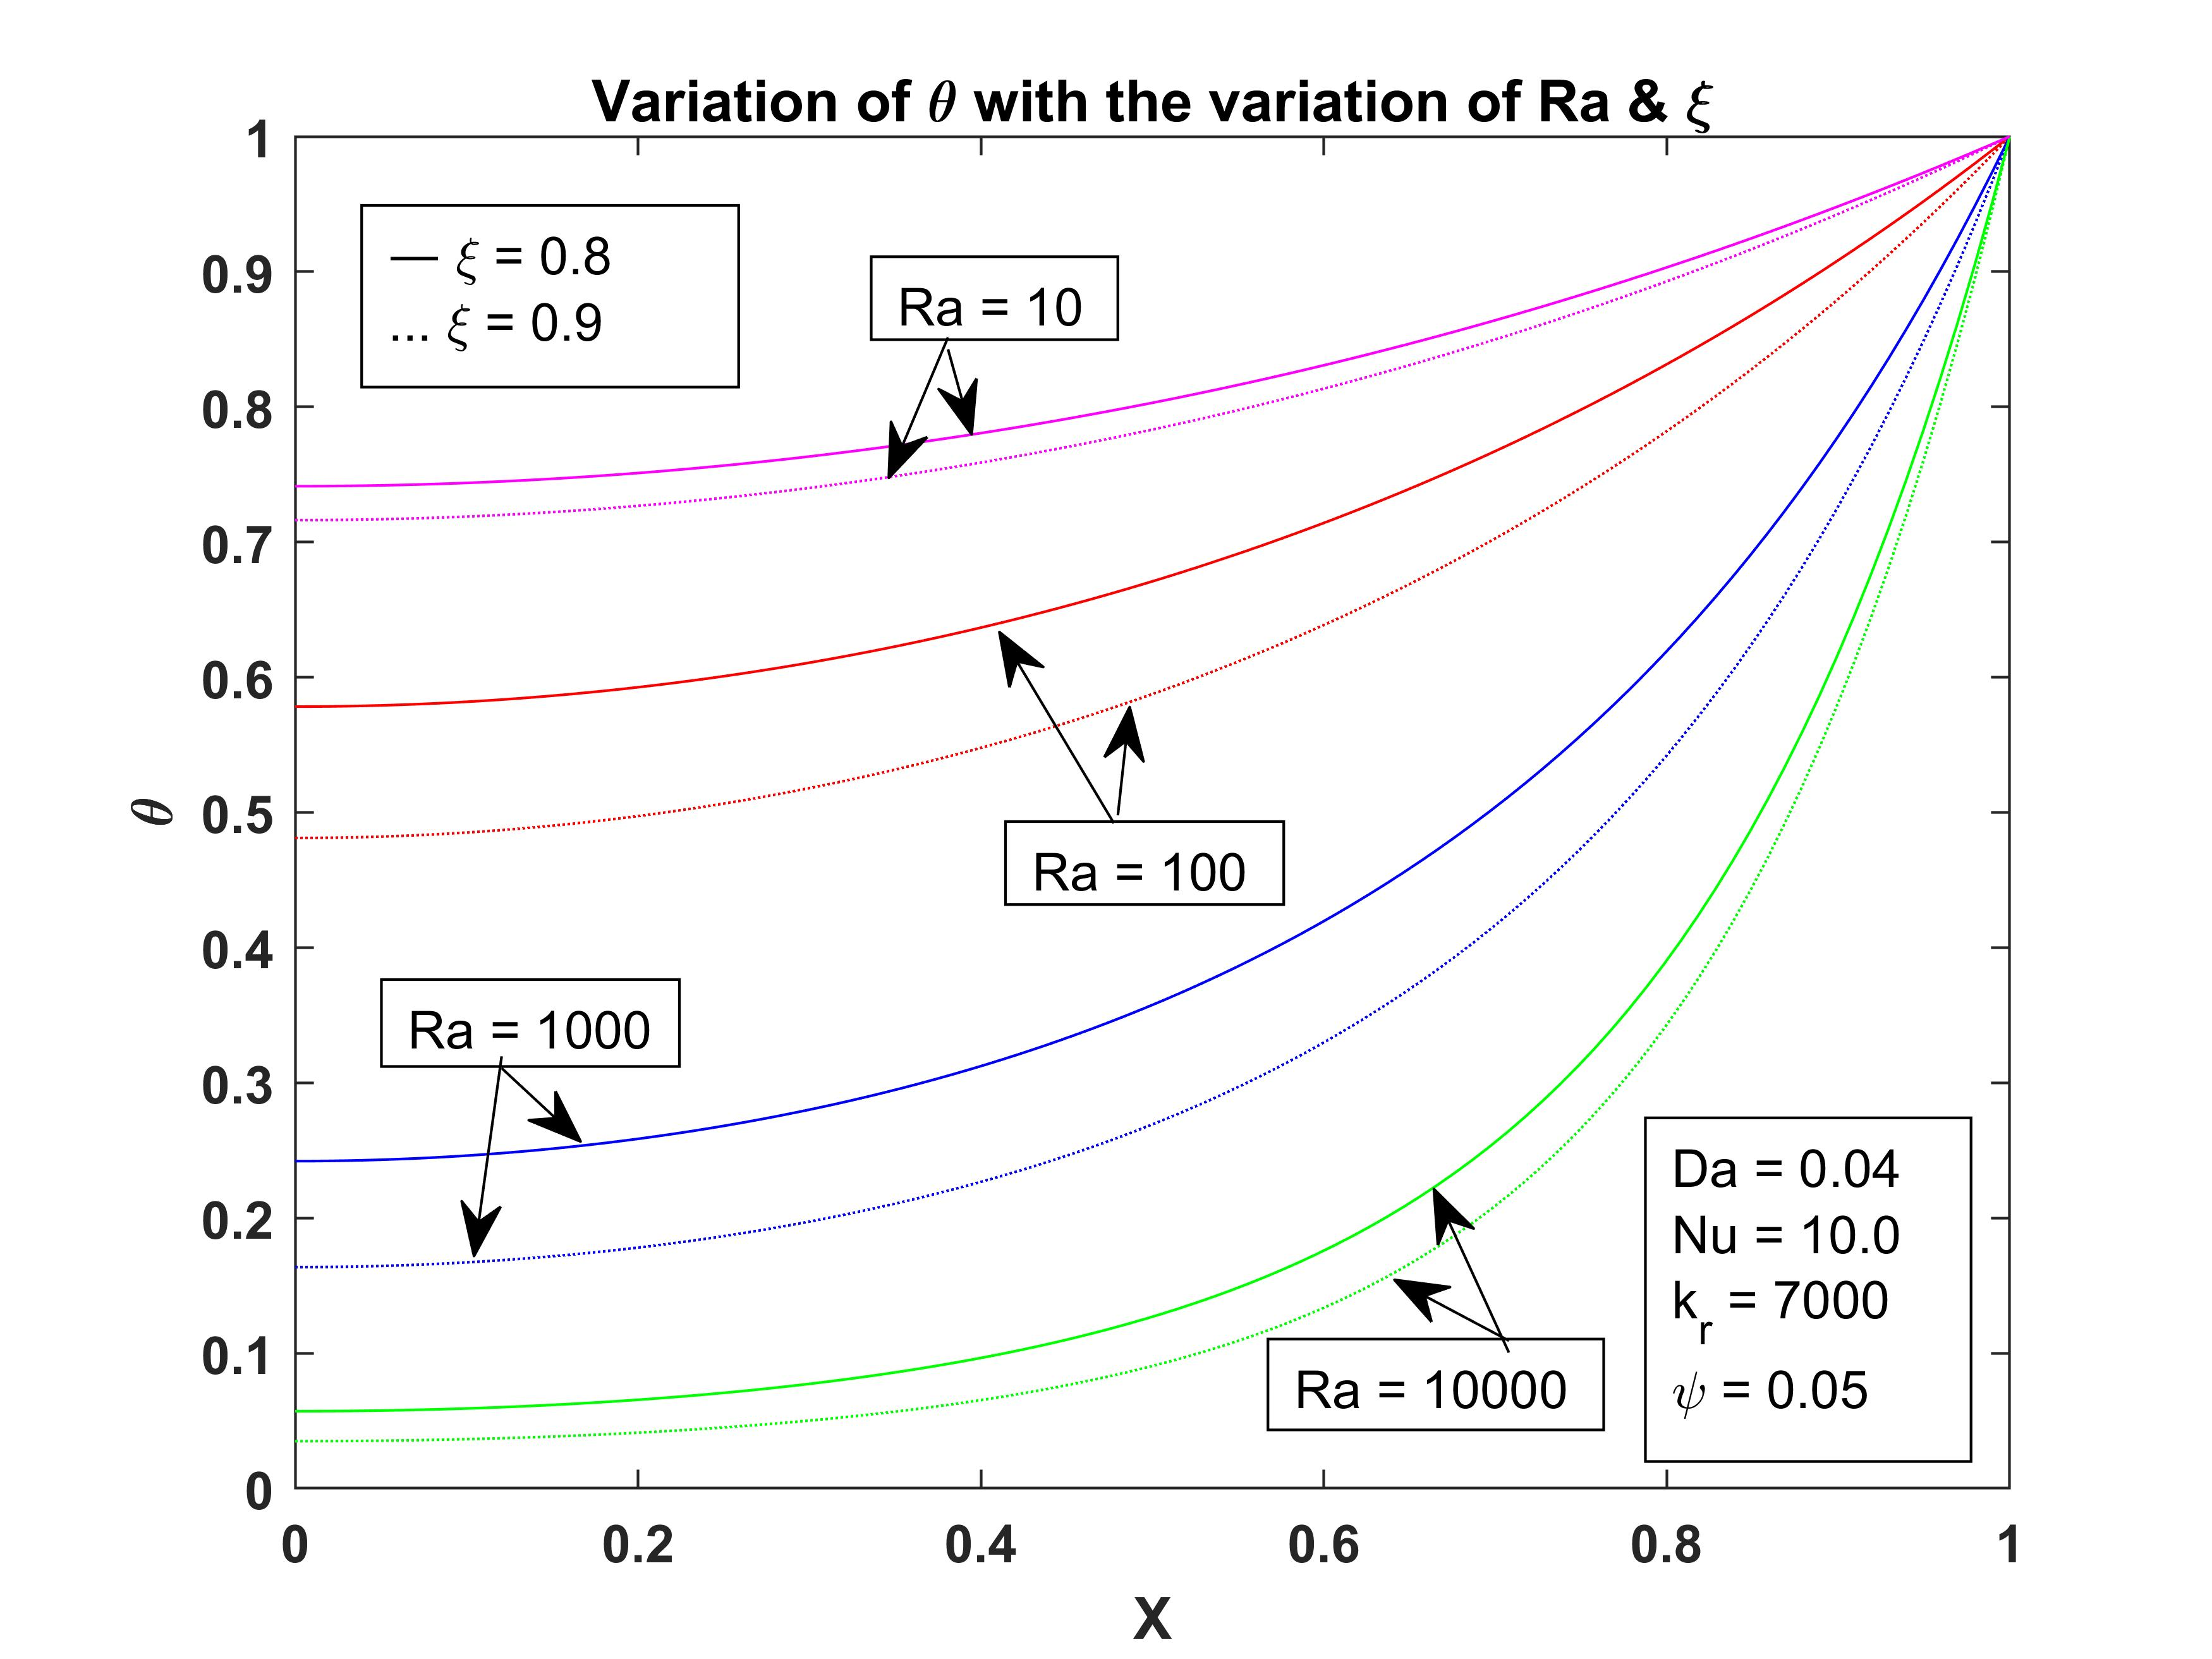
\includegraphics[scale=.08]{Analytical Solution/Fig 3a.jpg}
  \label{fig:5}
\end{minipage}
\end{figure}

\begin{figure}[H]
\begin{minipage}{.5\textwidth}
  \hspace{-1.4cm}
  \vspace{-1.4cm}
  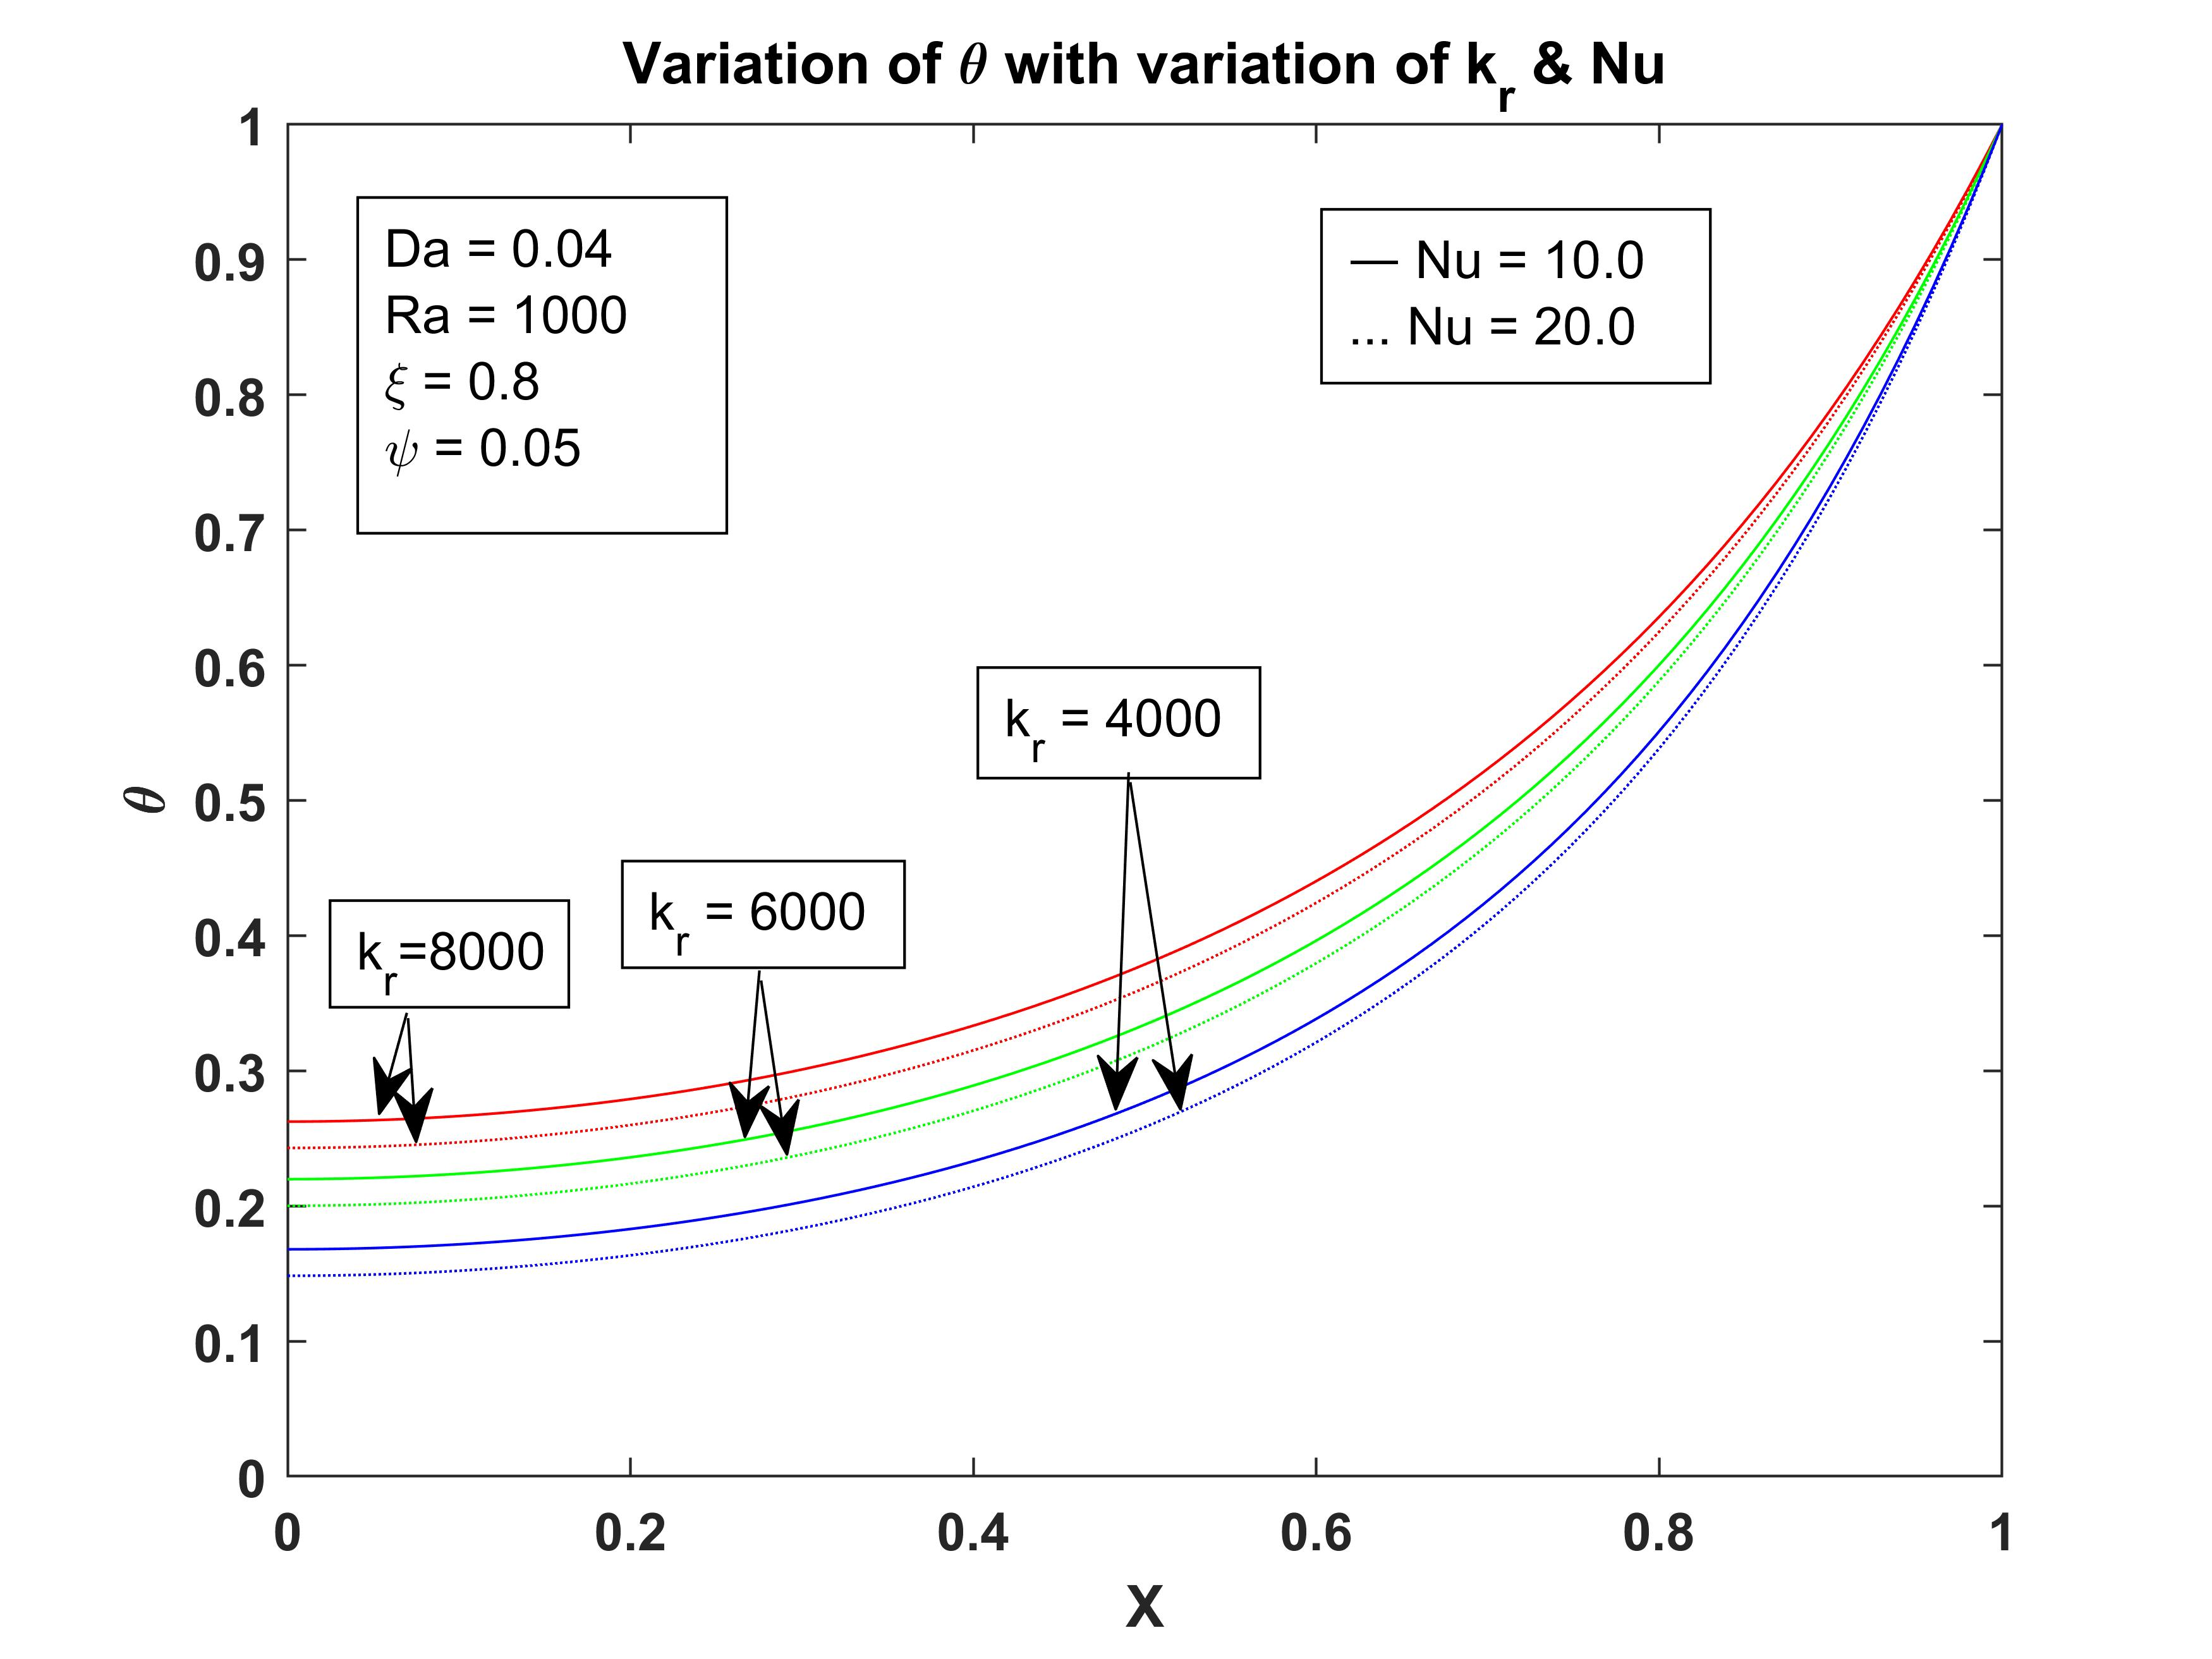
\includegraphics[scale=0.08]{Analytical Solution/Fig3b.jpg}
  \label{fig:6}
\end{minipage}%
\begin{minipage}{.5\textwidth}
  \hspace{-0.5cm}
   \vspace{-1.4cm}
  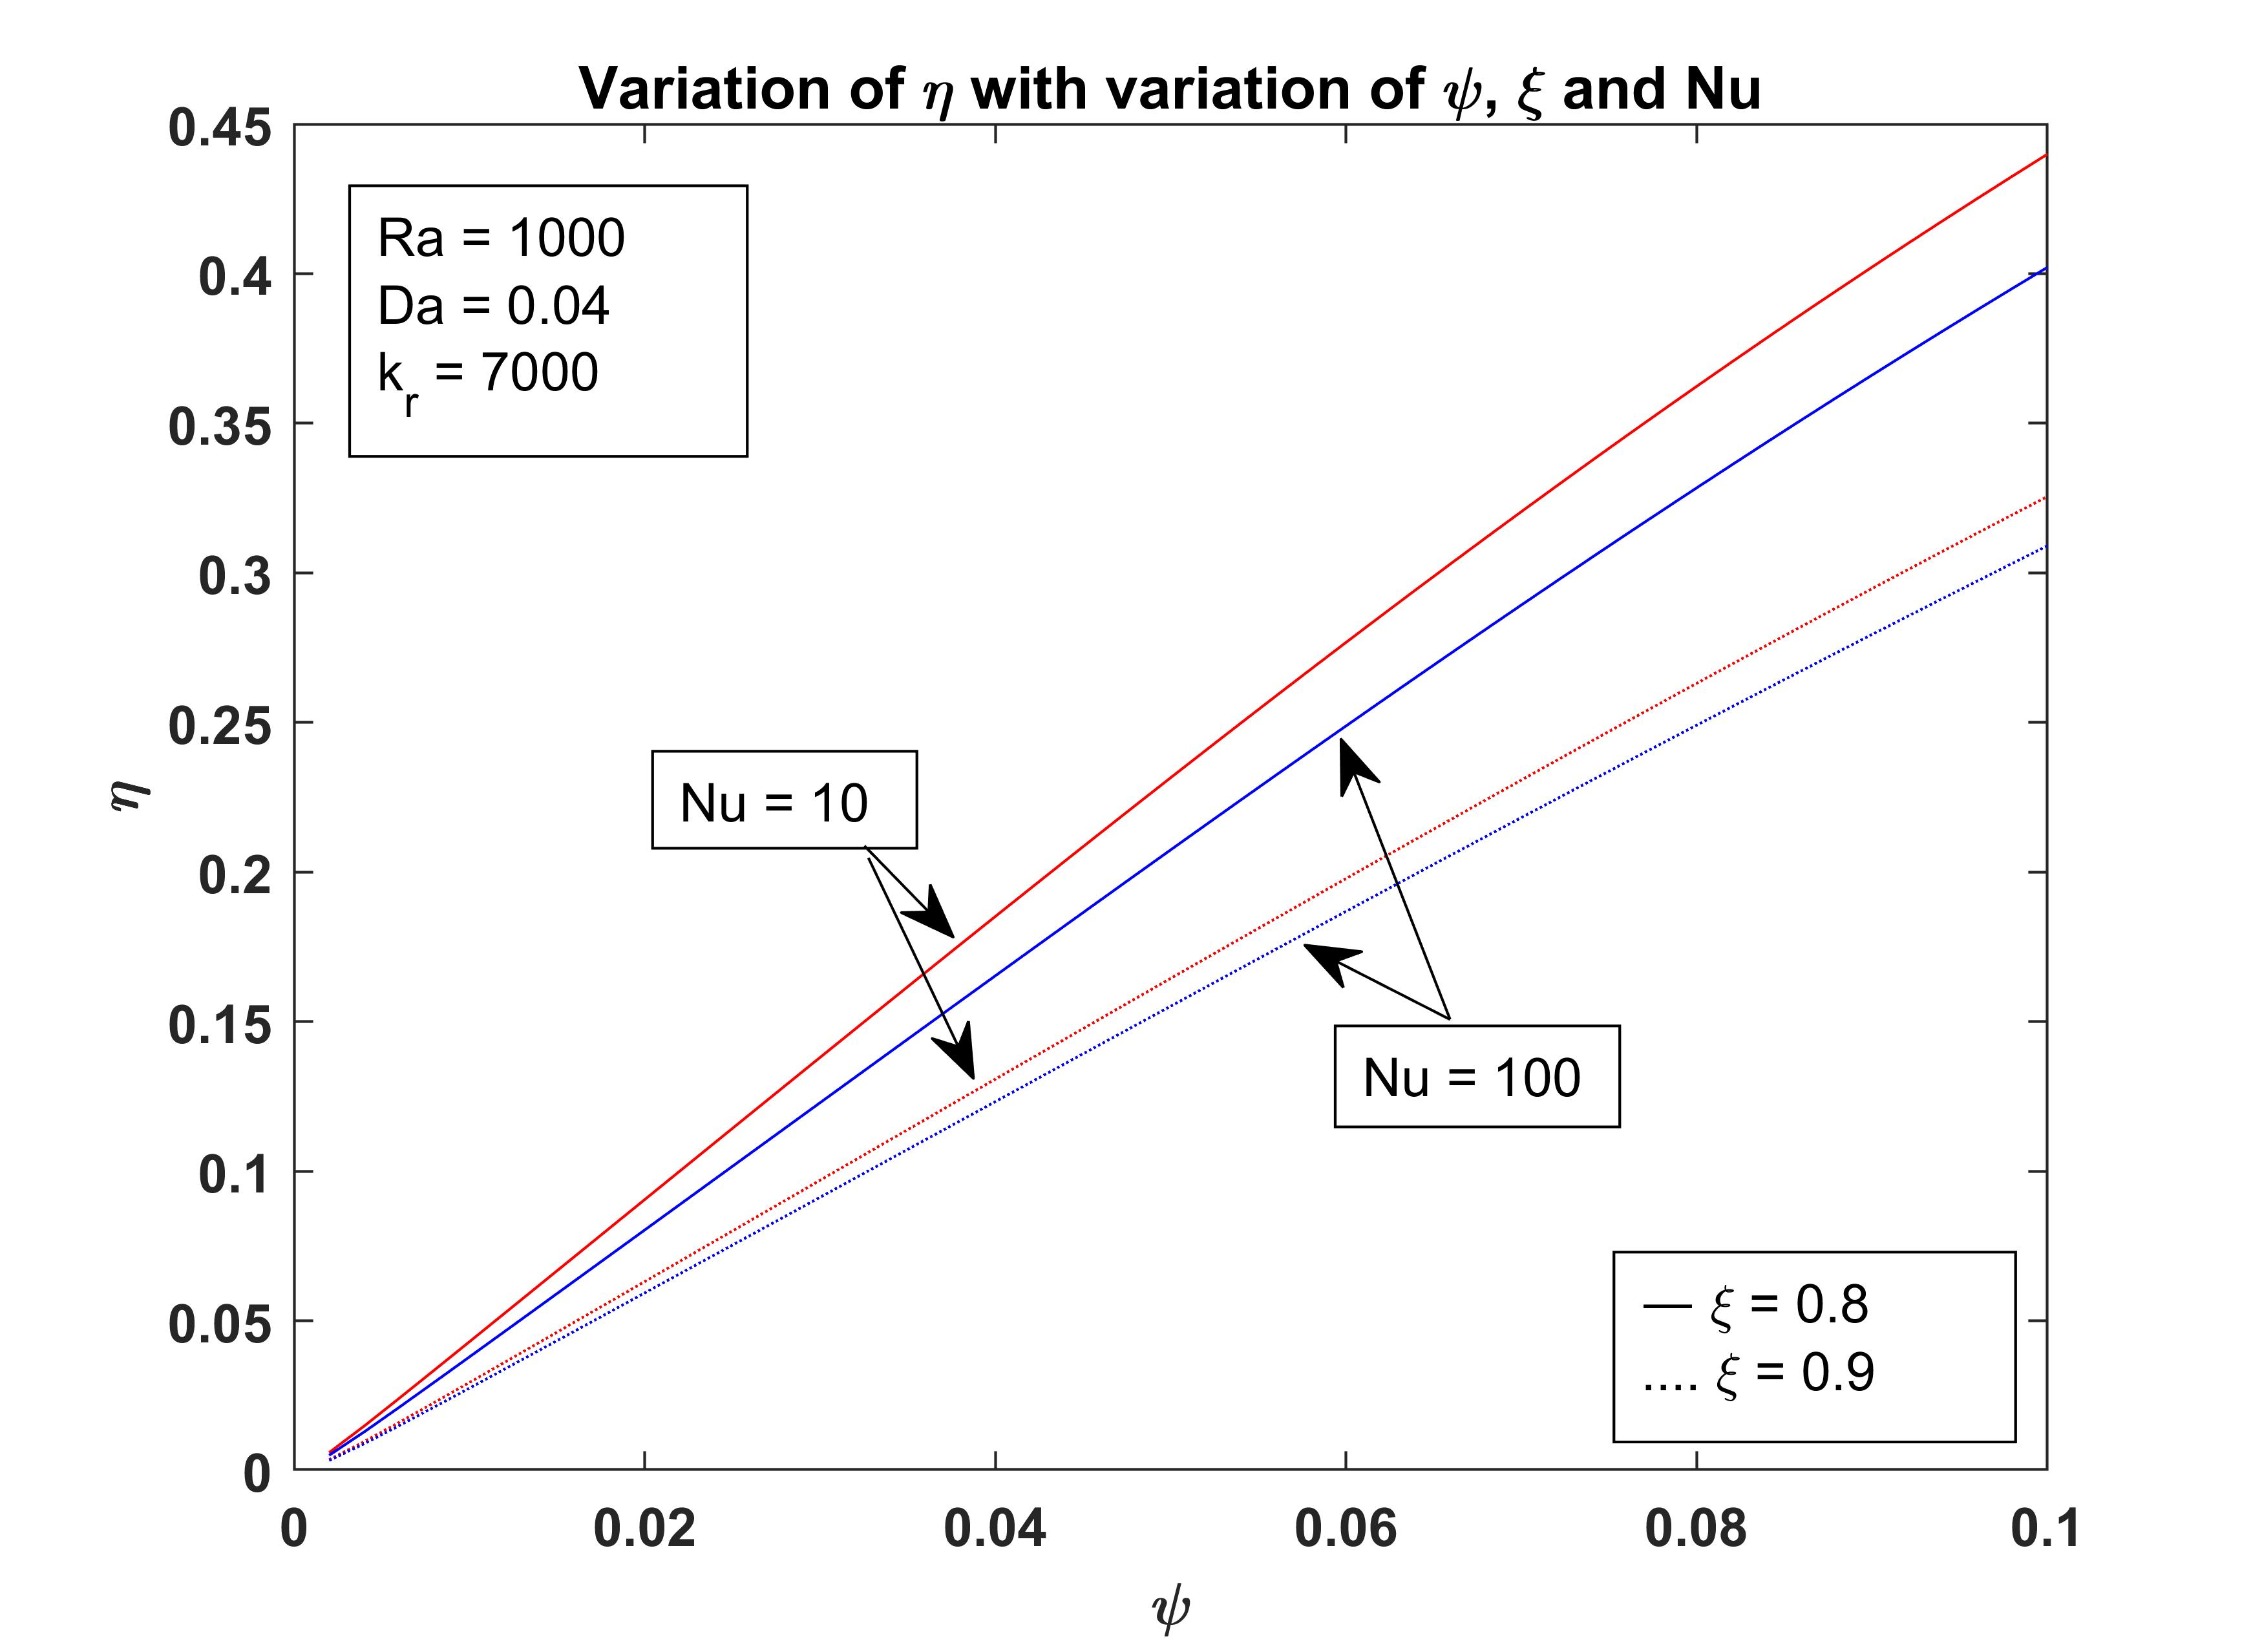
\includegraphics[scale=.08]{Analytical Solution/Fig4a.jpg}
  \label{fig:7}
\end{minipage}
\end{figure}

\begin{figure}[H]
\begin{minipage}{.5\textwidth}
  \hspace{-1.4cm}
  \vspace{-1.4cm}
  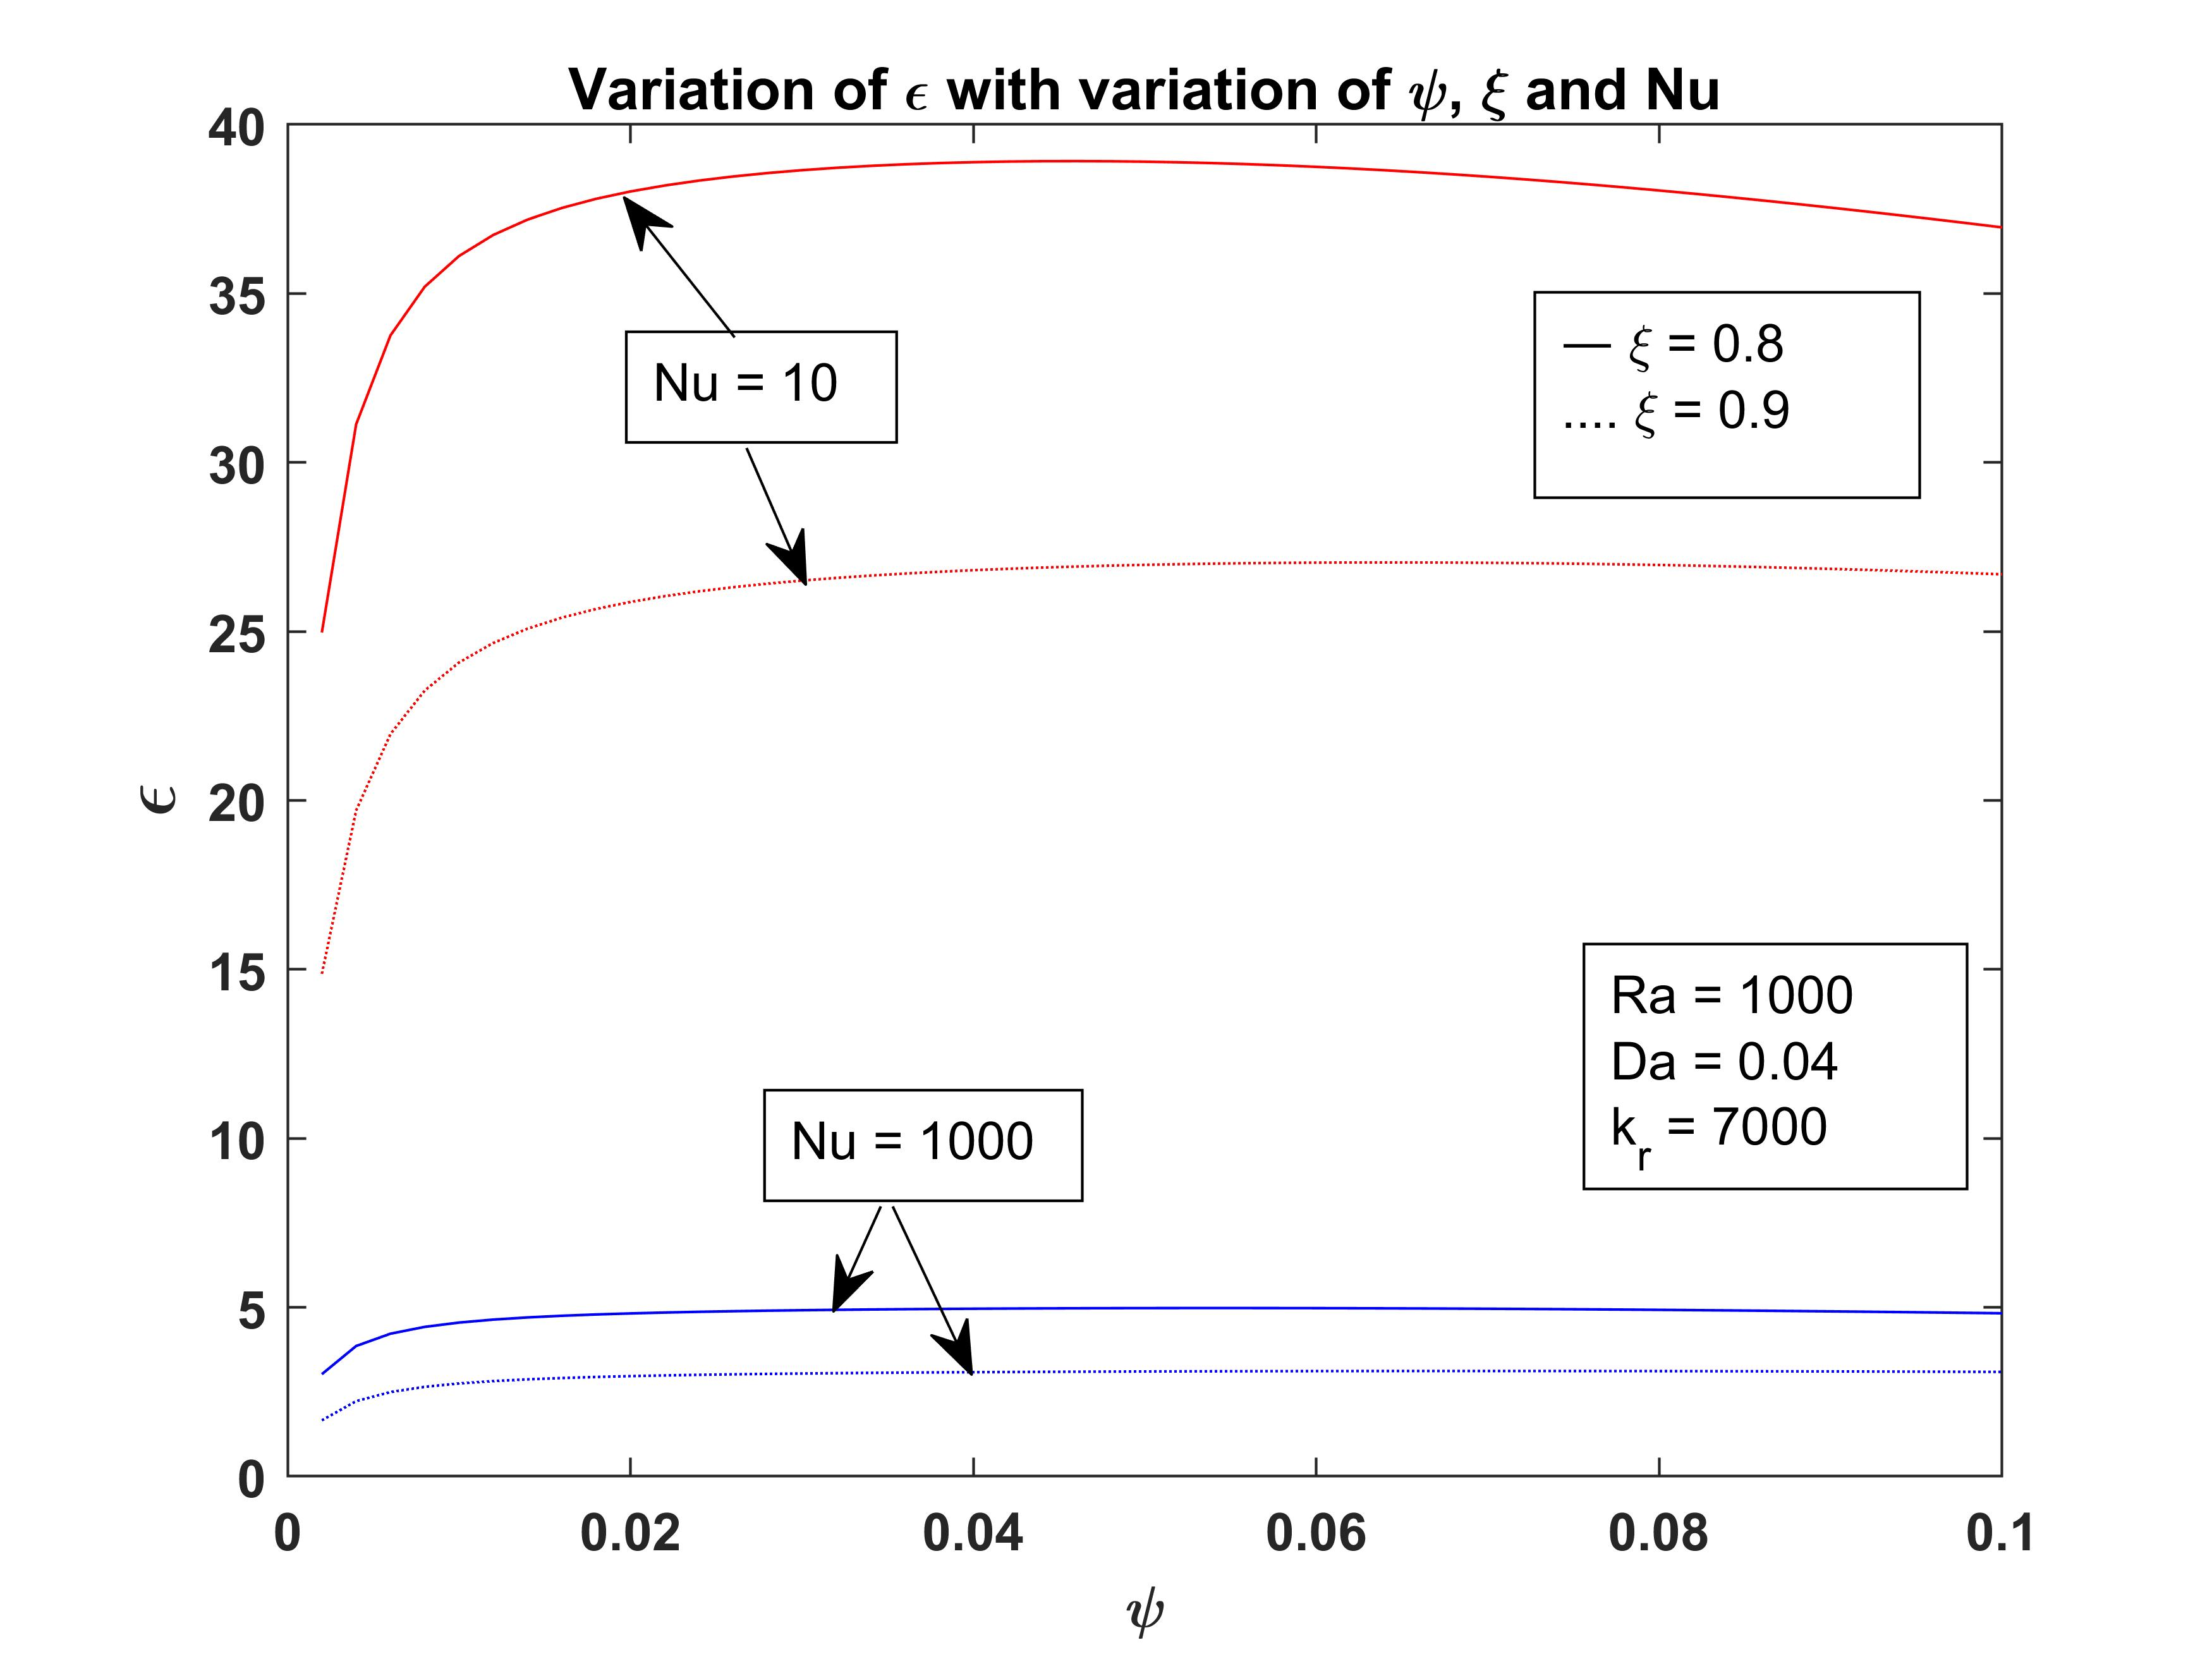
\includegraphics[scale=0.08]{Analytical Solution/Fig4b.jpg}
  \label{fig:8}
\end{minipage}%
\begin{minipage}{.5\textwidth}
  \hspace{-0.5cm}
  \vspace{-1.4cm}
  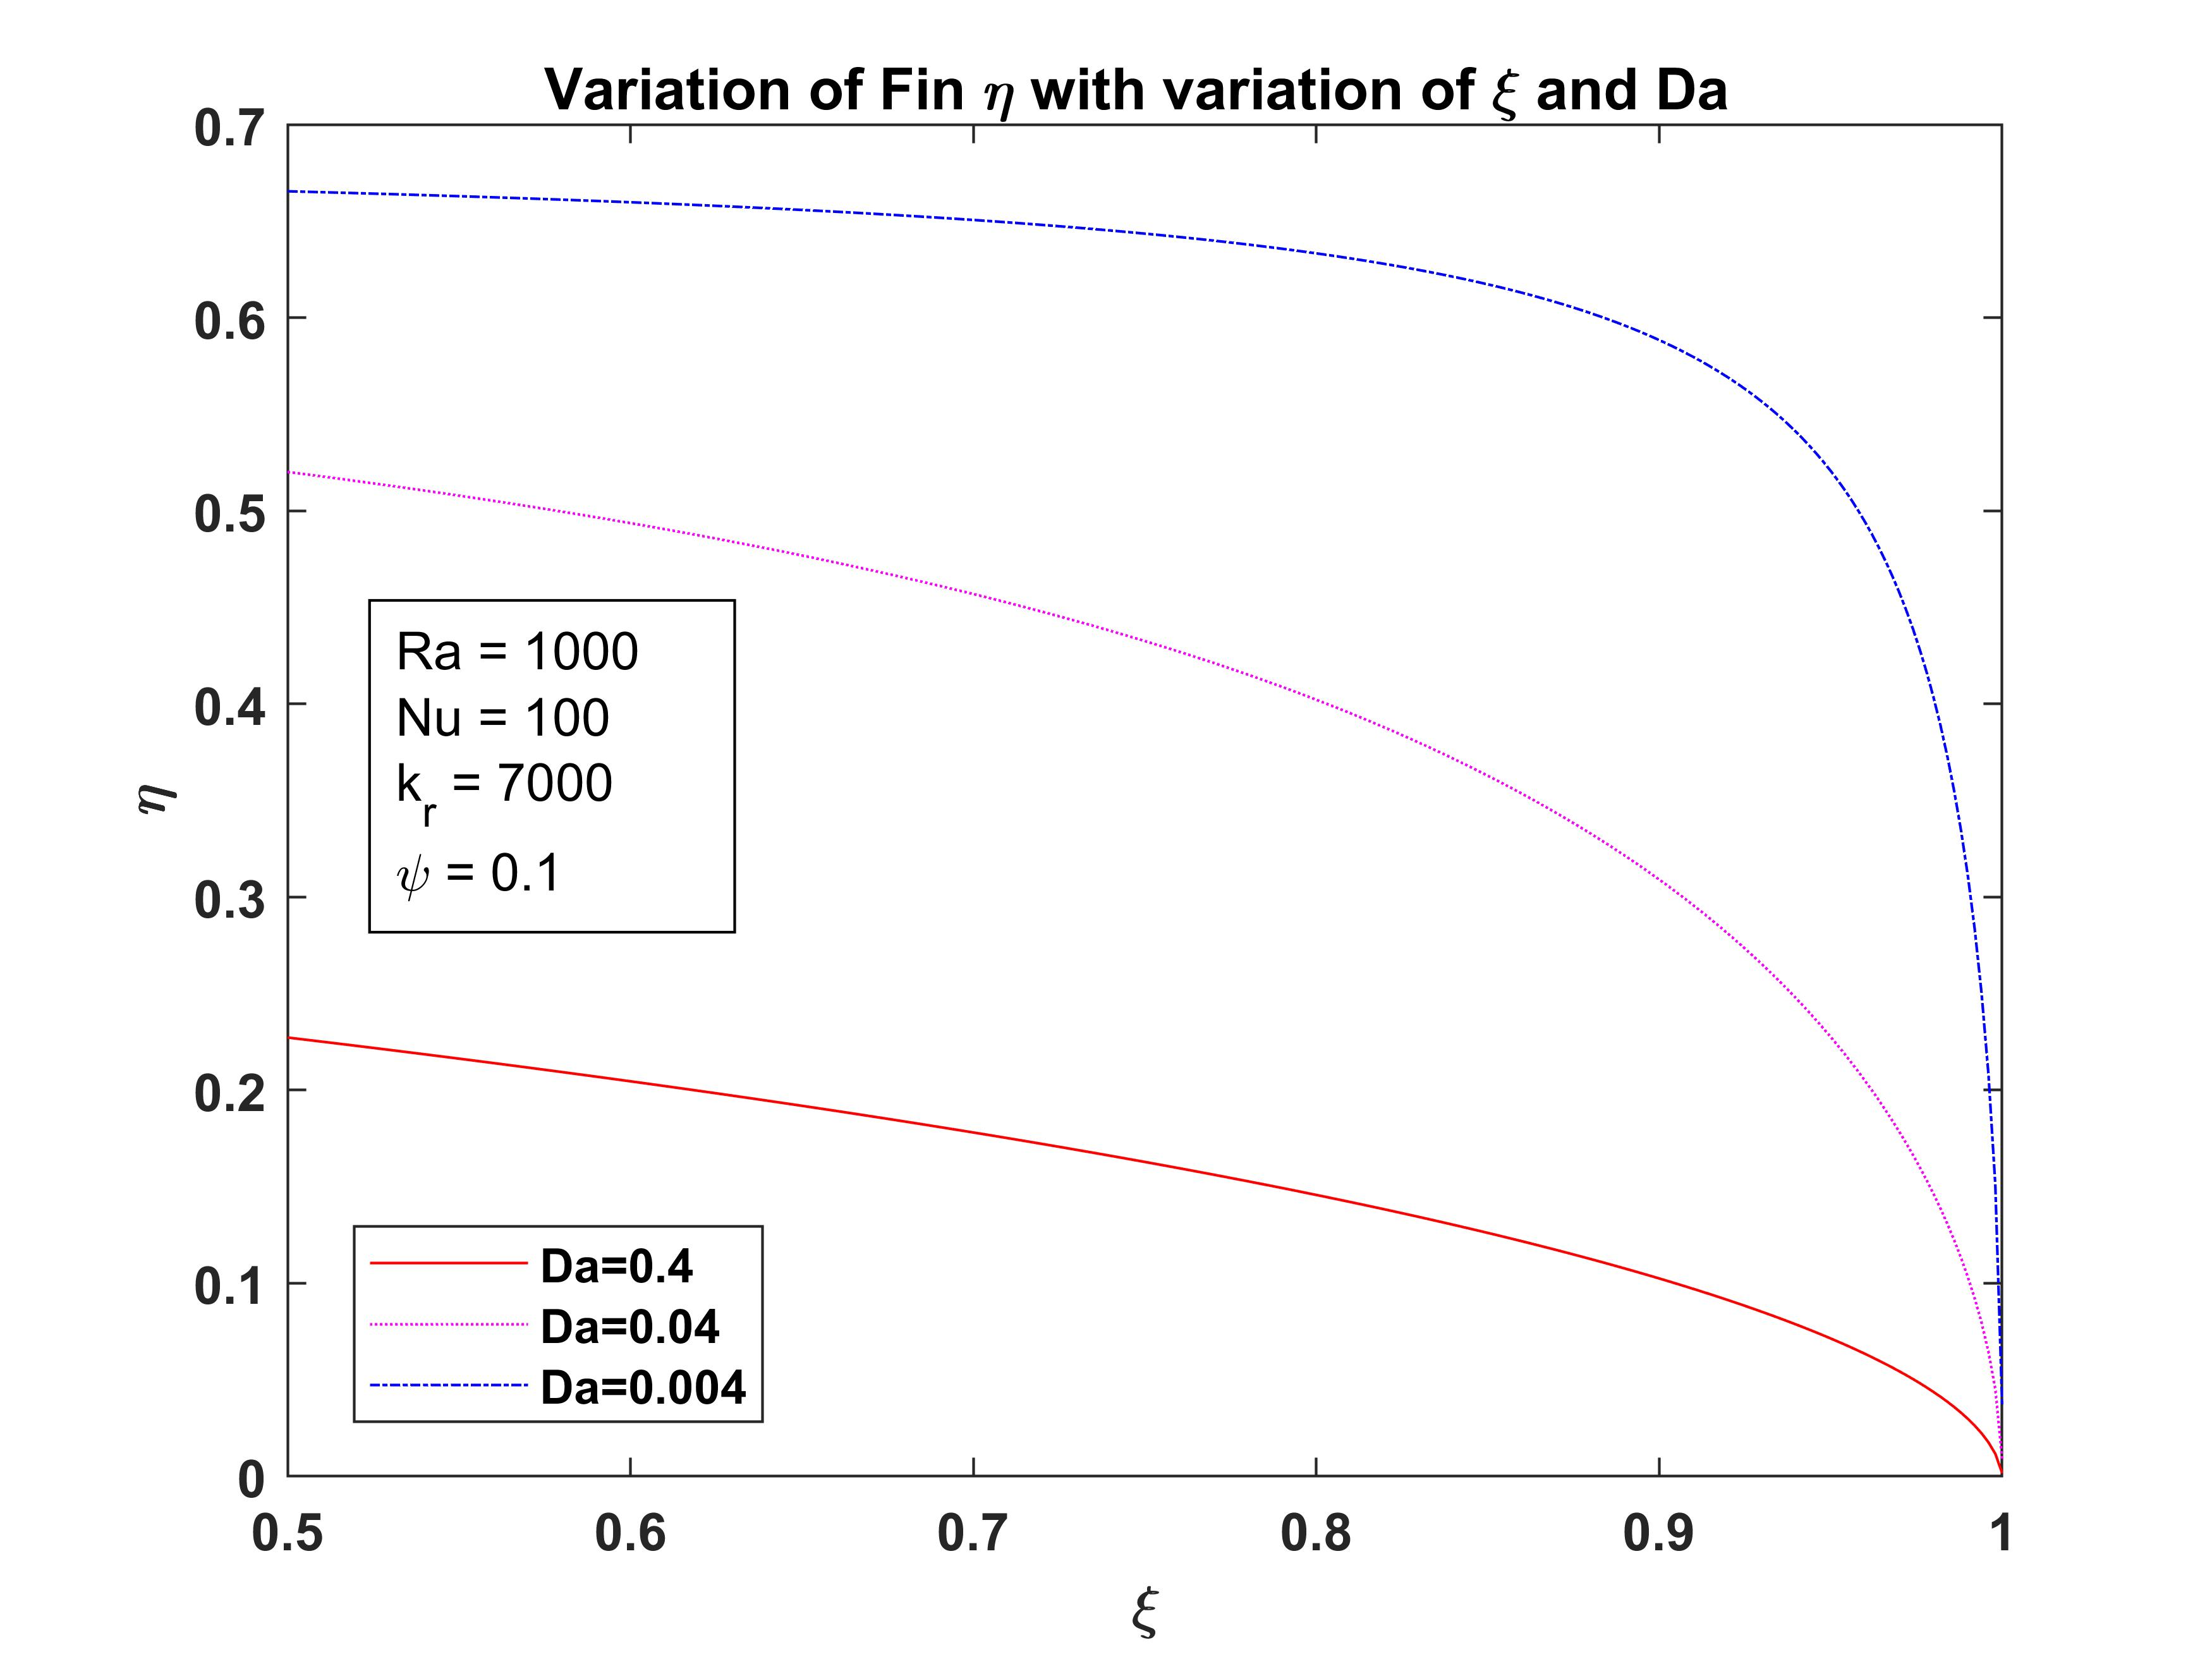
\includegraphics[scale=.08]{Analytical Solution/Fig5a.jpg}
  \label{fig:9}
\end{minipage}
\\ \\  
\caption{Results obtained from our MATLAB code}
\end{figure}

\section{Numerical Methods}
\subsection{Mesh}
The major part of the report focuses on the numerical approach to the ODE system presented previously. Our group has explored three main numerical methods, to serve as a means of validation of the results we obtain. Two of these are Finite Difference Methods (FDM) and the thrid is a Finite Volume Method (FVM). These are presented one by one with all the necessary detail in the subsequent sections. Before we delve into further detail, the computational grids and index notation followed for the FDM and the FVM solutions are presented below. The Finite Volume Method is implemented with cells of size $\Delta X \times 1 \times 1$ as it is a 1-D problem. 
\begin{figure}[H]
    \centering
    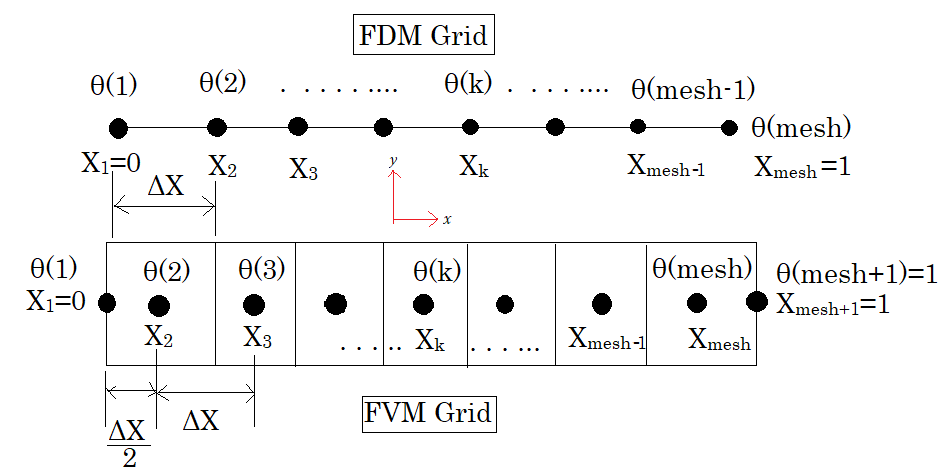
\includegraphics[scale=.8]{Description/Mesh.PNG}
    \caption{Grids for numerical methods used}
    \label{fig:10}
\end{figure}
\textbf{FVM Grid: }Notice that the FVM grid lies at the center of the imaginary cells, while the FDM nodes lie at the faces of the cells. Hence, the first $X$ coordinate of the FVM grid starts at $\frac{\Delta X}{2}$ ends at $1-\frac{\Delta X}{2}$. At the extreme ends are 0 and 1 respectively. Hence the $X$ array can be represented as: 
\[
X_{FVM} = \{0, \frac{\Delta X}{2}, \frac{3 \Delta X}{2}, .., 1-\frac{\Delta X}{2},1\}
\]
\textbf{FDM Grid: }This grid lies at the cell faces and is relatively simpler.The corresponding $X$ array for this method is:
\[
X_{FDM} = \{0, \Delta X, 2\Delta X,..,1-\Delta X, 1\}
\]
As any healthy numerical code behaves, the solution obtained from discretizing must be grid-independent after a point. This is inspected along with suitable error analysis in the subsequent sections to check consistency of the solutions we obtained. 
\subsection{Finite Difference Method - Non-Linear \footnote{shortened as FDM-NL henceforth}}
\subsubsection{Discretization}
The ODE represented by \eqref{9} is discretized using a second-order accurate central finite difference approximation for the second derivative in the LHS: 
\[
\frac{d^2\theta}{dX^2} = \frac{\theta_{i+1}+\theta_{i-1}-2\theta_i}{\Delta X^2} + \mathcal{O}(\Delta X^2) \tag{27} \label{27}
\]
Here the $i's$ represent the discretized spatial location.  Hence the above represents a 3-point spatial stencil. The RHS of the equation \eqref{9} is the embedded non-linearity, which is computed as:
\[
RHS = \omega_1 \theta_i^2 + \omega_2 \theta_i \tag{28} \label{28}
\]
Hence the discretized equation reads:
\[
 \frac{\theta_{i+1}+\theta_{i-1}-2\theta_i}{\Delta X^2} = \omega_1 \theta_i^2 + \omega_2 \theta_i \tag{29} \label{29}
\]
We now have a system of non-linear equations in the $\theta_i's$. We decided to solve the resulting system with the secant method: 
\[
x^{k+1} = \phi (x^k) \tag{30} \label{30}
\]
for the non-linear equation represented by:
\[
x = \phi (x) \tag{31} \label{31}
\]
Where $k$ represents the $k^{th}$ iteration. Following these lines of this, we use the following method for the resulting non-linear system: 
\[
\frac{\theta_{i+1}^k+\theta_{i-1}^k-2\theta_i^{k+1}}{\Delta X^2} = \omega_1 (\theta_i^k)^2 + \omega_2 \theta_i^{k+1} \tag{32} \label{32}
\]
Hence, collecting all the $\theta_i^{k+1}$'s to one side we get the update step of our algorithm, that relates the $i^{th}$ location of the $(k+1)^{th}$ iteration to the $k^{th}$ iteration values. 
\[
\theta_i^{k+1} = \frac{(\theta_{i+1}^k+\theta_{i-1}^k-\omega_1 h^2 (\theta_{i}^k)^2)}{2+\omega_2 h^2} \tag{33} \label{33}
\]
The boundary conditions for the problem are specified by \eqref{15} and \eqref{16}. The BC \eqref{15} can be trivially imposed by setting the ending value of the $\theta$ array to 1. The BC represented by \eqref{16} is imposed by backward finite difference approximation of the first derivative:
\[
\frac{\theta_2-\theta_1}{h} = 0 \label{34} \tag{34}
\]
Hence: 
\[
\theta_1 = \theta_2 \label{35} \tag{35}
\]
The above step has to performed after/before every update to the next iteration. This shall become clearer with the algorithm we present in the next section. It is to be noted that MATLAB arrays start with 1. Hence for $n$ points we have the $\theta$ array as: 
\[
[\theta] = \{\theta_1, \theta_2,...,\theta_n\} \tag{36} \label{36}
\]
Hence the mesh spacing $h$ becomes: 
\[
h = \frac{1}{n-1} \tag{37} \label{37}
\]
Because the total non-dimensionalized length is unity. A suitable stopping criterion based on the converegence can be:
\[
tol = \sum_{i=1}^n (\theta_i^{k+1} - \theta_i^k) \leq \epsilon \tag{38} \label{38}
\]
Where $\epsilon$ denotes the tolerance. 
\subsubsection{Algortithm}
\begin{enumerate}
    \item Read the inputs $Ra, Da, Nu, \xi, k_r, \psi$
    \item Compute $\omega_1$ and $\omega_2$ using \eqref{7}
    \item Read mesh size and compute $h$ from \eqref{37}
    \item Declare the $\theta$ array and set $\theta(end)=1$
    \item Begin the outer $k$ loop and repeat 6,7 until $\epsilon<tol$
    \item Until $(i<n)$ do \eqref{33} starting from $i=2$
    \item set the BC \eqref{35}
    \item if $\epsilon<tol$ exit and plot
\end{enumerate}
\subsubsection{Implementation}
The above algorithm is implemented as a segmented code with functions for computing the parameters of the ODE, performing the NL-FDM on the $\theta$ array. The NL-FDM function takes the 3 inputs namely the parameter array containing the constants to calculate $\omega$'s, the mesh size and the tolerance for the secant method. Results have been presented for the cases indicated in the paper with tight tolerances of upto $10^{-10}$ indicating excellent convergence. The following figure shows the call-graph for the $``main.m"$ file which houses all the solvers in one place:
\begin{figure}[H]
    \centering
    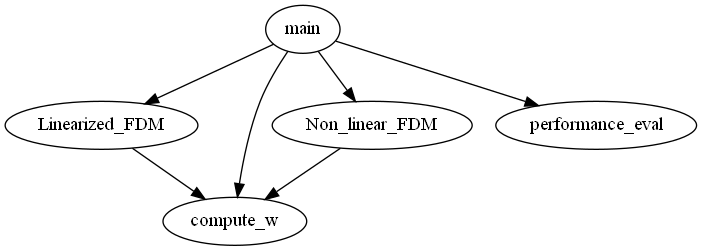
\includegraphics[scale=.5]{Call graphs/Main_call_graph.png}
    \caption{Call graph for the master file}
    \label{fig:11}
\end{figure}
\subsubsection{Results and validation}
\subsubsubsection{Agreement with analytical solutions}
The results obtained from FDM are compared each time with the analytical solution. The details of the parameters chosen can be found in the figures themselves. As visible from these plots, excellent agreement between them is observed validating both our NL-FDM solution approach and the analytical solution.
\begin{figure}[H]
\begin{minipage}{.5\textwidth}
    \hspace{-1.4cm}
    \vspace{-1.4cm}
  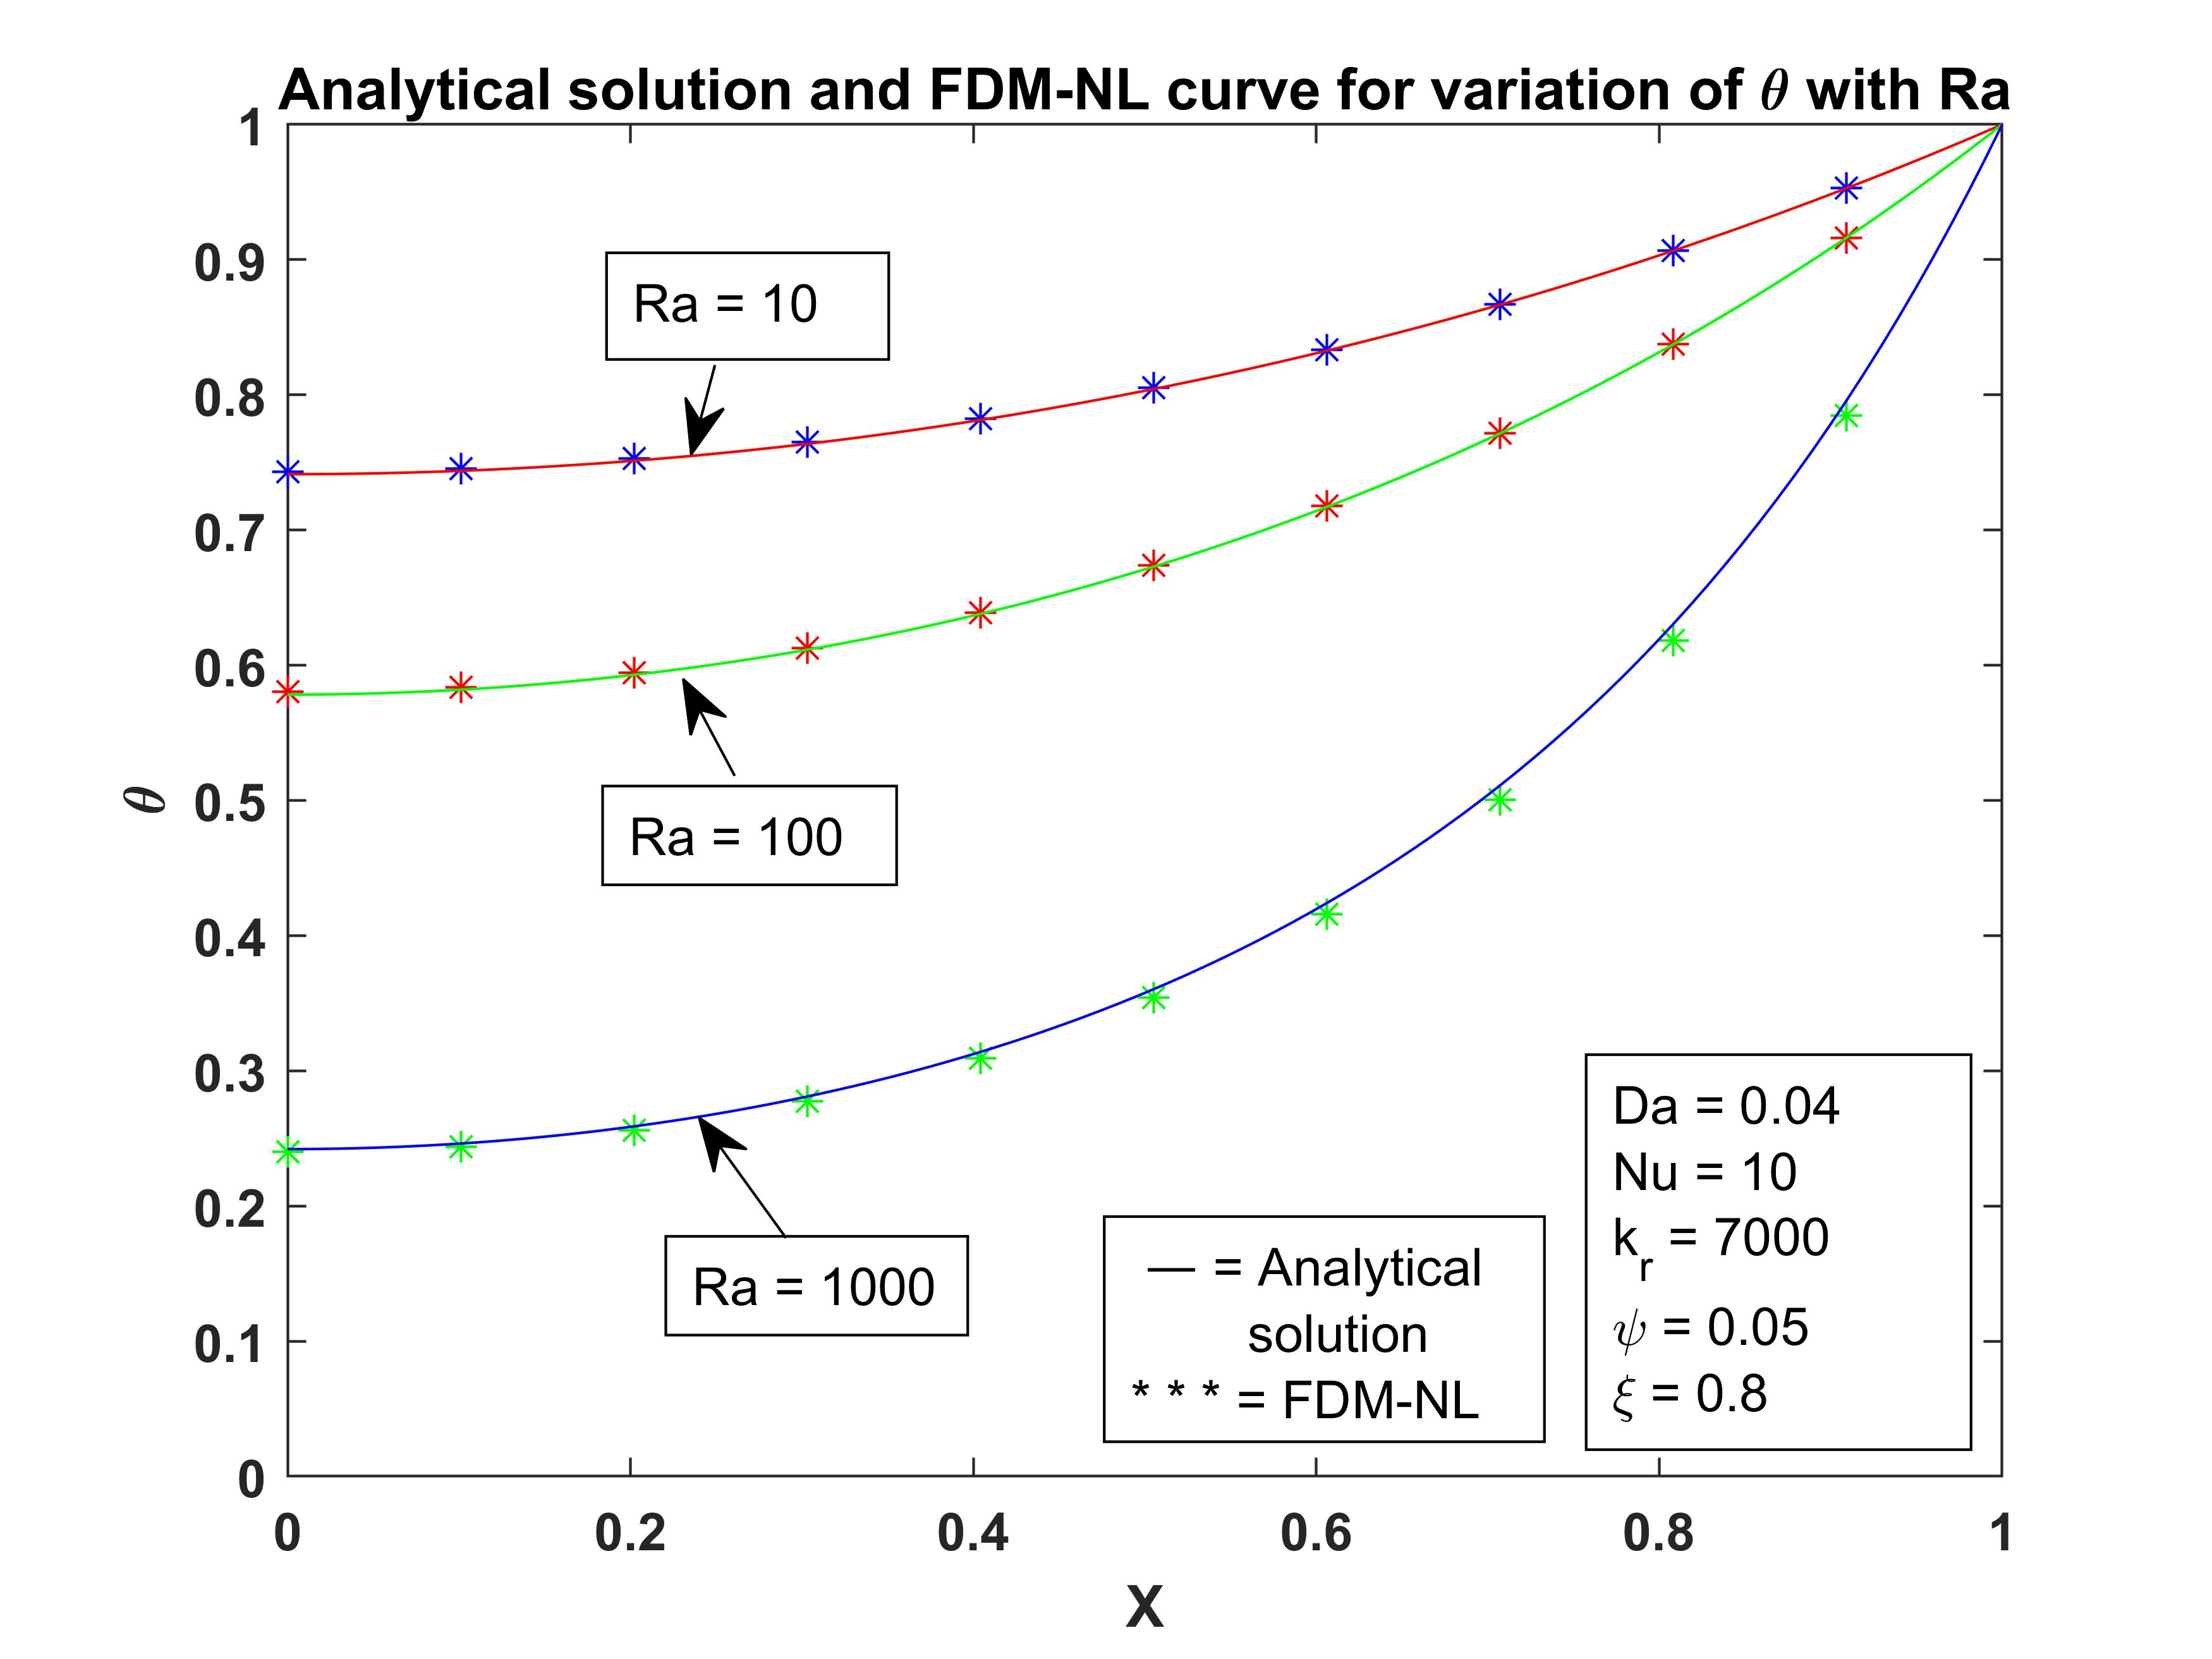
\includegraphics[scale=0.08]{Numerical Methods/NLFDM/FDM NL Fig3a.jpg}
  \label{fig:12}
\end{minipage}%
\begin{minipage}{.5\textwidth}
  \hspace{-0.5cm}
  \vspace{-1.4cm}
  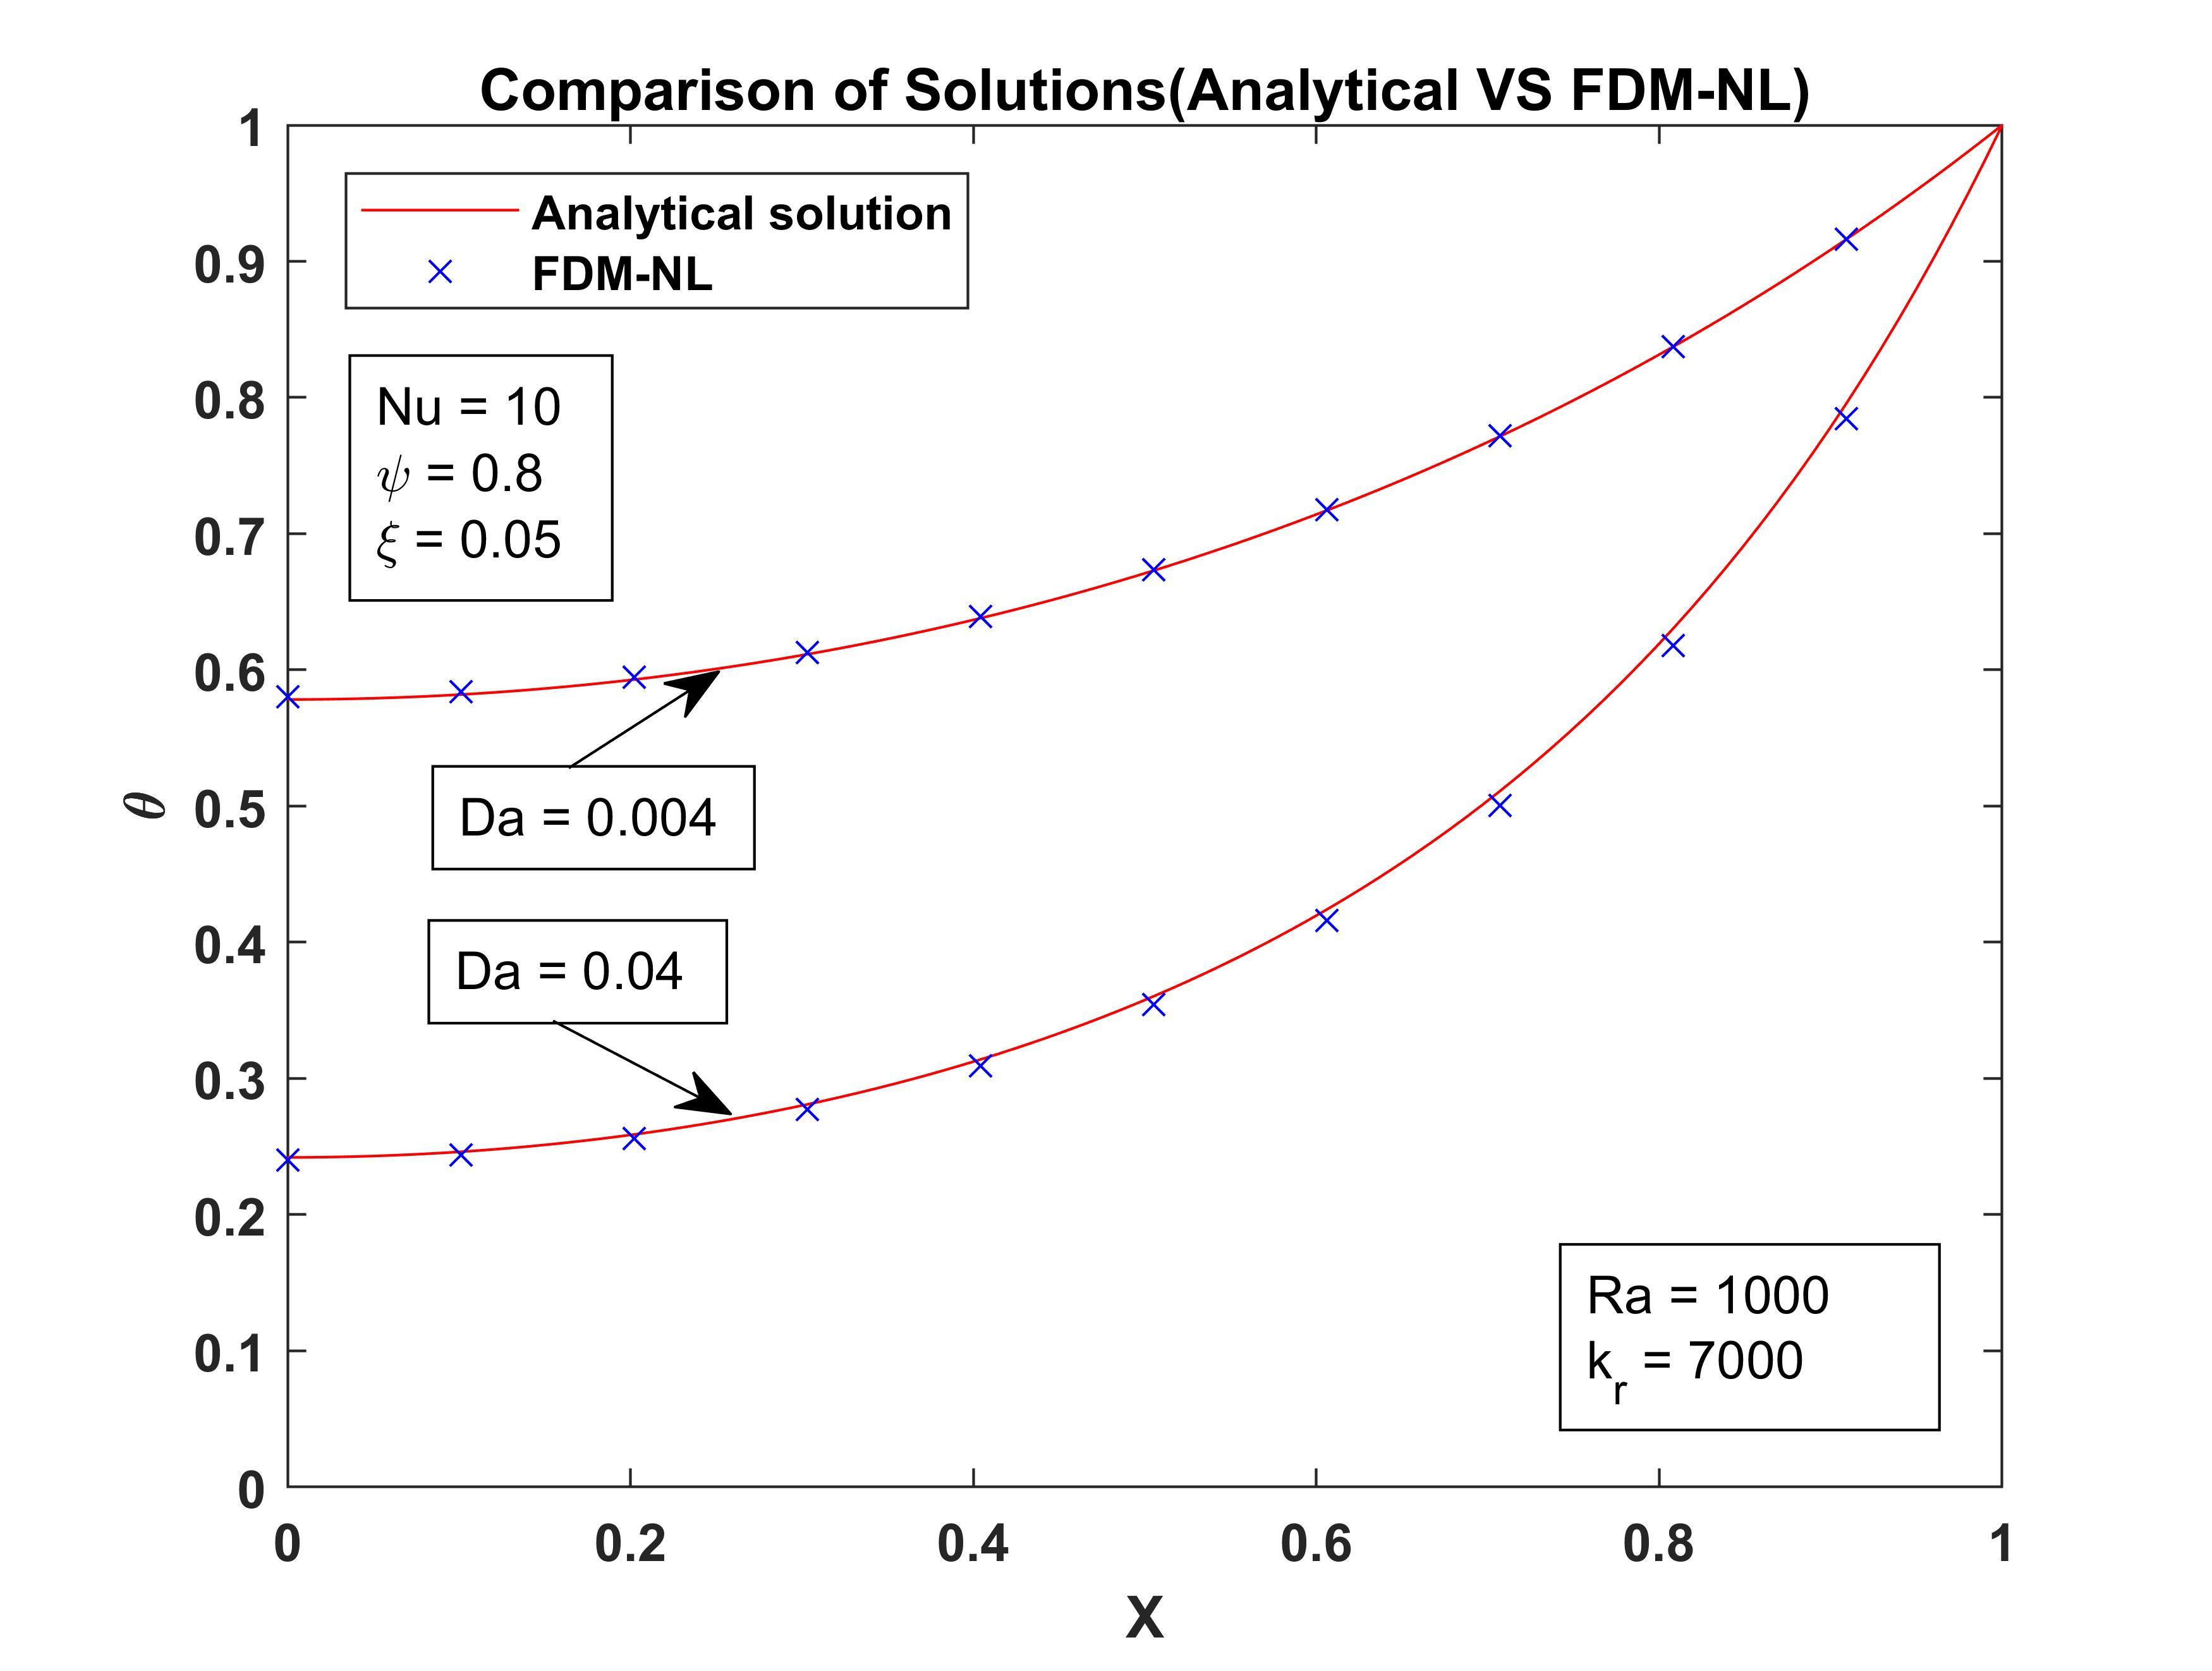
\includegraphics[scale=.08]{Numerical Methods/NLFDM/FDM NL.jpg}
  \label{fig:13}
\end{minipage}
\\ \\ 
\caption{Agreement with analytical solution}
\end{figure}
\subsubsubsection{Inspecting accuracy}
To further investigate the accuracy of the code hence obtained, we decided to inspect the deviation of the two results by varying the $Ra$ parameter keeping others constant: 
\[
\{k_r,\xi, Da, Nu, \psi, mesh, tol\} = \{7000,0.8,0.004,0.05,100,10^{-10}\}
\]
The $Ra$ value is varied from 100 to 10000 in appropriate steps.From the graphs presented its evident that at larger Rayleigh numbers there is greater deviation. The group feels that is an error in the way the analytical solution is approximated rather than the numerical result due to the usage of a fixed number of adomain polynomials. The error at a computed as:
\[
\delta \theta_i = \frac{\theta^{analytical}_i-\theta^{FDM/FVM}_i}{\theta^{analytical}_i}
\]
Hence the mean error is:
\[
\delta \theta_{mean} = \sum_i^{Mesh} \delta \theta_i
\]

\begin{figure}[H]
\begin{minipage}{.5\textwidth}
    \hspace{-1.4cm}
    \vspace{-1.4cm}
  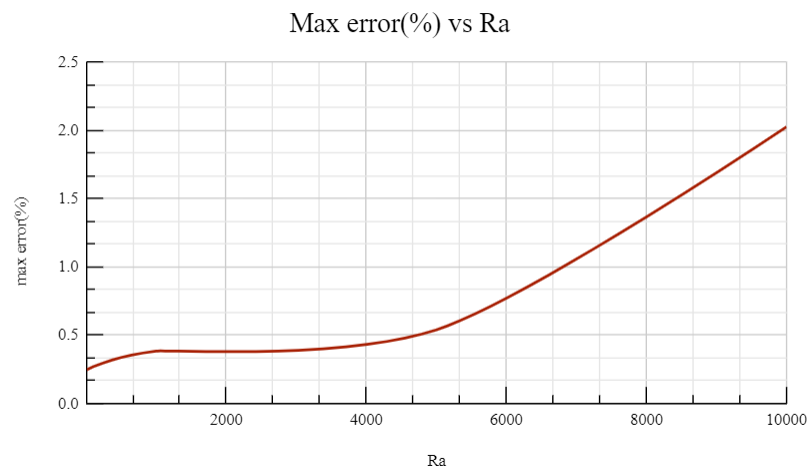
\includegraphics[scale=0.5]{Numerical Methods/NLFDM/Max_error_Ra.PNG}
  \label{fig:14}
\end{minipage}%
\begin{minipage}{.5\textwidth}
  \hspace{-0.5cm}
  \vspace{-1.4cm}
  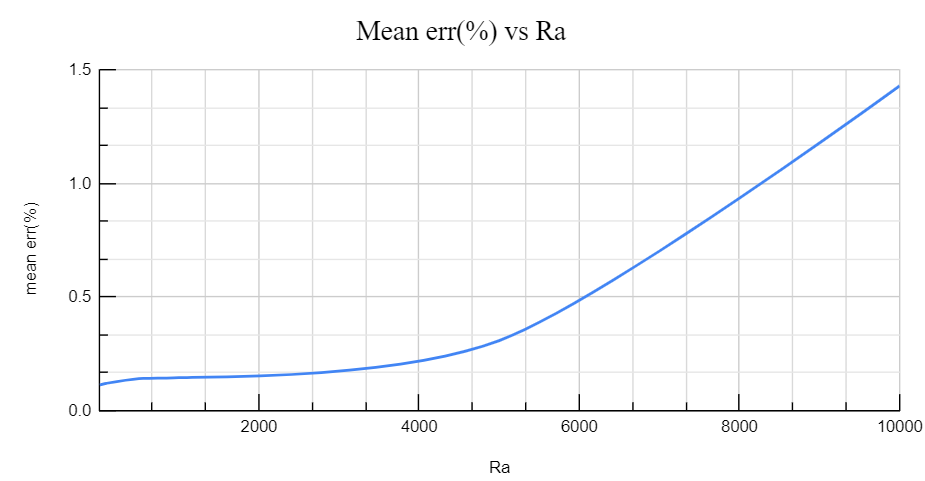
\includegraphics[scale=.5]{Numerical Methods/NLFDM/Mean_error_Ra.PNG}
  \label{fig:15}
\end{minipage}
\\ \\ 
\caption{Mean error for high Ra is only 1.5\%}
\end{figure}

The in built MATLAB profiler was used to find out the time taken by the code to run. The solver run time and the total time of the program are hence obtained and plotted: 

\begin{figure}[H]
\begin{minipage}{.5\textwidth}
    \hspace{-0.4cm}
    \vspace{-1.4cm}
  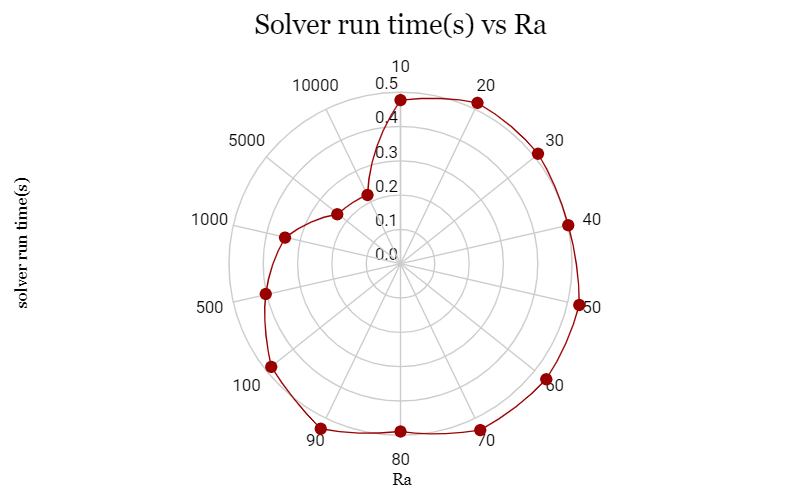
\includegraphics[scale=0.5]{Numerical Methods/NLFDM/Solver_run_time_Ra.PNG}
  \label{fig:16}
\end{minipage}%
\begin{minipage}{.5\textwidth}
  \hspace{-0.5cm}
  \vspace{-1.4cm}
  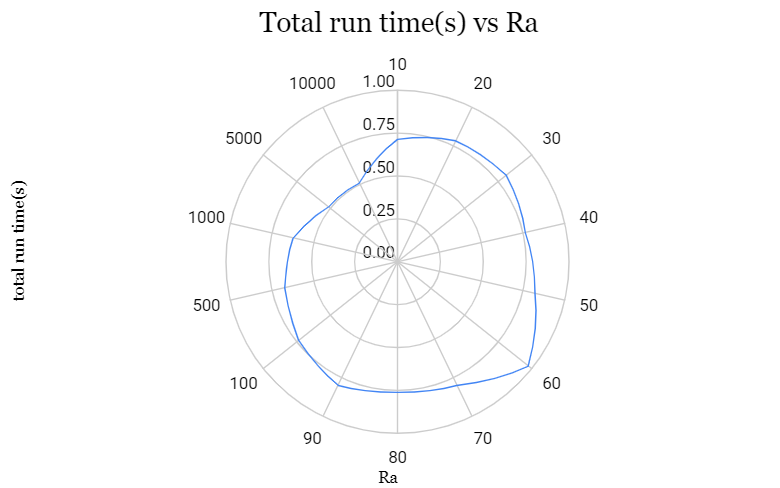
\includegraphics[scale=.5]{Numerical Methods/NLFDM/Total_run_time_Ra.PNG}
  \label{fig:17}
\end{minipage}
\\ \\ \\ \\
\caption{At higher Ra lower run times were observed}
\end{figure}

The same was conducted for other parameters as well namely for $k_r,Da,\psi,Nu,\xi$ and much deviation wasn't observed from the analytical solution. The datasets are available as \href{https://docs.google.com/spreadsheets/d/14CD9h_oIQvpSYWhHdYkxh0rk-RfhSL3lAaR-XjAy2KA/edit?usp=sharing}{Google sheets} and the reader can refer the same. For the sake of conciseness this is avoided in the report. Also, since the solutions match for $\theta-X$ graphs with the analytical, the performance parameters were also found to be identical to the analytical solution and this too is skipped.
\subsubsubsection{Grid Independence}
We inspected grid-independence on the following set of inputs: 
\[
\{k_r,\xi, Da, Nu, \psi, Ra, tol\} = \{7000,0.8,0.004,0.05,100,10^{-10}\}
\]
It was found that the same holds good for other inputs.The solver run time, total run time, the mean error from the analytical solution and the value of $\theta(1)$ (the value at the pin base) was noted for the mesh sizes ranging from 100 to 1000. The results are presented below: 

\begin{figure}[H]
\begin{minipage}{.5\textwidth}
    \hspace{-0.4cm}
    \vspace{-1.4cm}
  \includegraphics[scale=0.5]{Numerical Methods/NLFDM/Mean_error_mesh.PNG}
  \label{fig:18}
\end{minipage}%
\begin{minipage}{.5\textwidth}
  \hspace{0.7cm}
  \vspace{-1.4cm}
  \includegraphics[scale=.5]{Numerical Methods/NLFDM/theta_mesh.PNG}
  \label{fig:19}
\end{minipage}
\\ \\ \\ \\
\caption{(Left)Error reduces with increasing mesh size. (Right) $\theta(1)$ is close to a perfect circle indicating there is little effect of the grid size on the solution. }
\end{figure}

\begin{figure}[H]
\begin{minipage}{.5\textwidth}
    \hspace{-0.4cm}
    \vspace{-1.4cm}
  \includegraphics[scale=0.5]{Numerical Methods/NLFDM/Solver_run_mesh.PNG}
  \label{fig:20}
\end{minipage}%
\begin{minipage}{.5\textwidth}
  \hspace{0.7cm}
  \vspace{-1.4cm}
  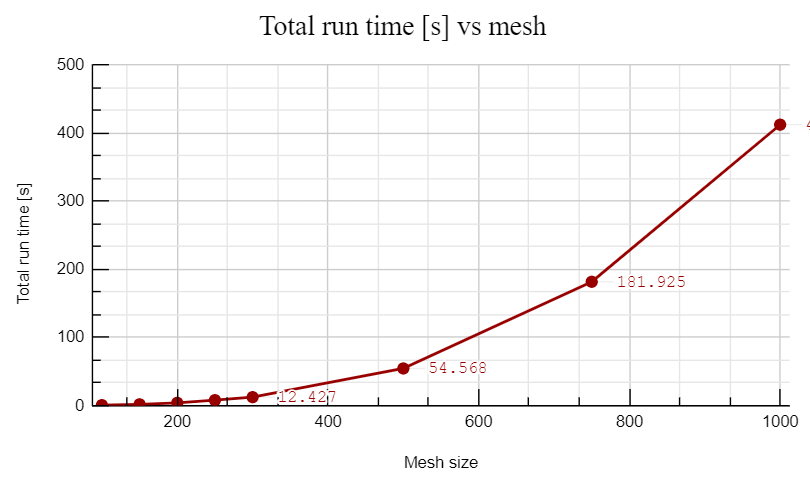
\includegraphics[scale=.5]{Numerical Methods/NLFDM/Total_run_mesh.PNG}
  \label{fig:21}
\end{minipage}
\\ \\ \\ \\
\caption{(Left) Solver run time exponentially increases. (Right) Solver run time occupies the 99\% of the total time}
\end{figure}

From these results we infer that the solver we coded is robust and behaves as expected. The small deviations that have been observed are because of errors in discretization and error in the analytical solution due to the number of adomain polynomials used. Sample data: 
{\begin{center}
\begin{tabularx}{0.8\textwidth} { 
  | >{\raggedright\arraybackslash}X 
  | >{\centering\arraybackslash}X 
  | >{\raggedleft\arraybackslash}X 
  | >{\raggedleft\arraybackslash}X |}
 \hline
 Mesh & Mean error[\%] & $\theta(1)$ & Run time [s] \\
 \hline
 100 & 0.1205  & 0.7433 & 0.729 \\
\hline
 200 & 0.05975 & 0.7423 & 4.105 \\
\hline
 300 & 0.039677 & 0.7421 & 12.122 \\
\hline
 500 & 0.02370 & 0.7420 & 54.252\\
\hline
 1000 & 0.0117 & 0.7415 & 412.42\\
 \hline
\end{tabularx}
\end{center}
}
\subsection{Finite Difference Method - Linearized}
\subsubsection{Discretization}
The discretization for this method is exactly the same as the previous section until we reach equation \eqref{31}. However, the secant method is applied in a different way on the RHS of \eqref{32} for the non-linear term $\theta_i^2$. We adopt a splitting of the power between the previous iteration and the next iteration as follows:
\[
\frac{\theta_{i+1}^k+\theta_{i-1}^k-2\theta_i^{k+1}}{\Delta X^2} = \omega_1 \theta_i^k \theta_i^{k+1} + \omega_2 \theta_i^{k+1} \tag{39} \label{39}
\]
Once again collecting all the $\theta_i^{k+1}$'s to one side we obtain the modified loop update as follows: 
\[
\theta_i^{k+1}=\frac{\theta_{i+1}^k + \theta_{i-1}^k - (\omega_2 h^2)\theta_i^k}{2 + \theta_i^k \omega_1 h^2} \label{40} \tag{40}
\]
Rest everything remains the same as the previous method. 
\subsubsection{Algortithm}
\begin{enumerate}
    \item Read the inputs $Ra, Da, Nu, \xi, k_r, \psi$
    \item Compute $\omega_1$ and $\omega_2$ using \eqref{7}
    \item Read mesh size and compute $h$ from \eqref{37}
    \item Declare the $\theta$ array and set $\theta(end)=1$
    \item Begin the outer $k$ loop and repeat 6,7 until $tol<\epsilon$
    \item Until $(i<n)$ do \eqref{40} starting from $i=2$
    \item set the BC \eqref{35} 
    \item if $tol<\epsilon$ exit and plot results
\end{enumerate}
\subsubsection{Implementation}
Implementation of the linearized FDM was done on the same lines as that of the non-linear FDM. A generic function with the 3 input paramters (constants, mesh and the tolerance) is constructed in MATLAB so that it can be as generalized as possible. The same code organization is followed (further details can be found in section \ref{sec:Code}). Also in order to evaluate performance parameters of the fin, the obtained temperature distribution, mesh and the constants are sent as inputs to another function, that returns the effectiveness, efficiency and the heat transfer rate. 
\subsubsection{Results and validation}
\subsubsubsection{Accuracy}
Excellent agreement is obtained between all three methods listed so far. The plots show how the linearized and non-linearized versions compare and it is apparent they are identical. Nonetheless we decided to compute the error and it was zero everywhere (right).

\begin{figure}[H]
\begin{minipage}{.5\textwidth}
    \hspace{-0.2cm}
    \vspace{-1.4cm}
  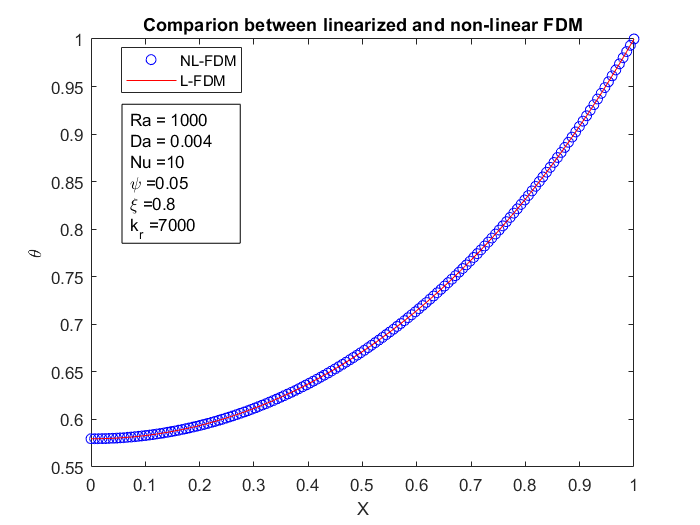
\includegraphics[scale=0.5]{NL_L_compare.png}
  \label{fig:22}
\end{minipage}%
\begin{minipage}{.5\textwidth}
  \hspace{0.0cm}
  \vspace{-1.4cm}
  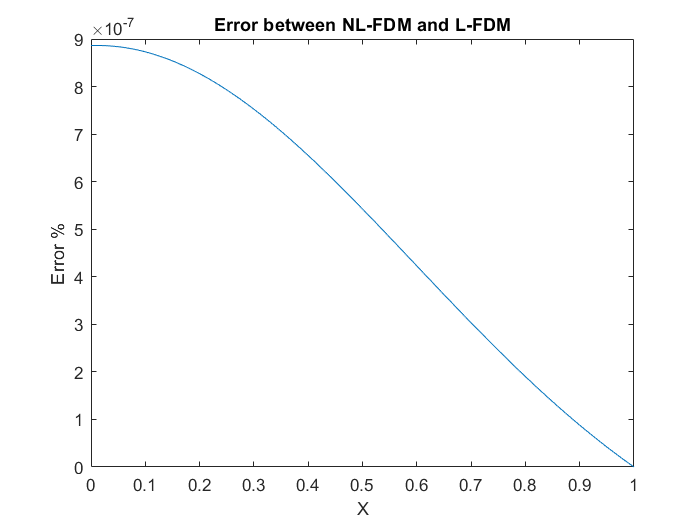
\includegraphics[scale=.5]{error_NL_L.png}
  \label{fig:23}
\end{minipage}
\\ \\
\caption{(Left) Identical results obtained (Right) Error \% of the order of $10^{-7}$}
\end{figure}

We now compare them with the analytical solution for different cases:

\begin{figure}[H]
\begin{minipage}{.5\textwidth}
    \hspace{-0.5cm}
    \vspace{-1.4cm}
  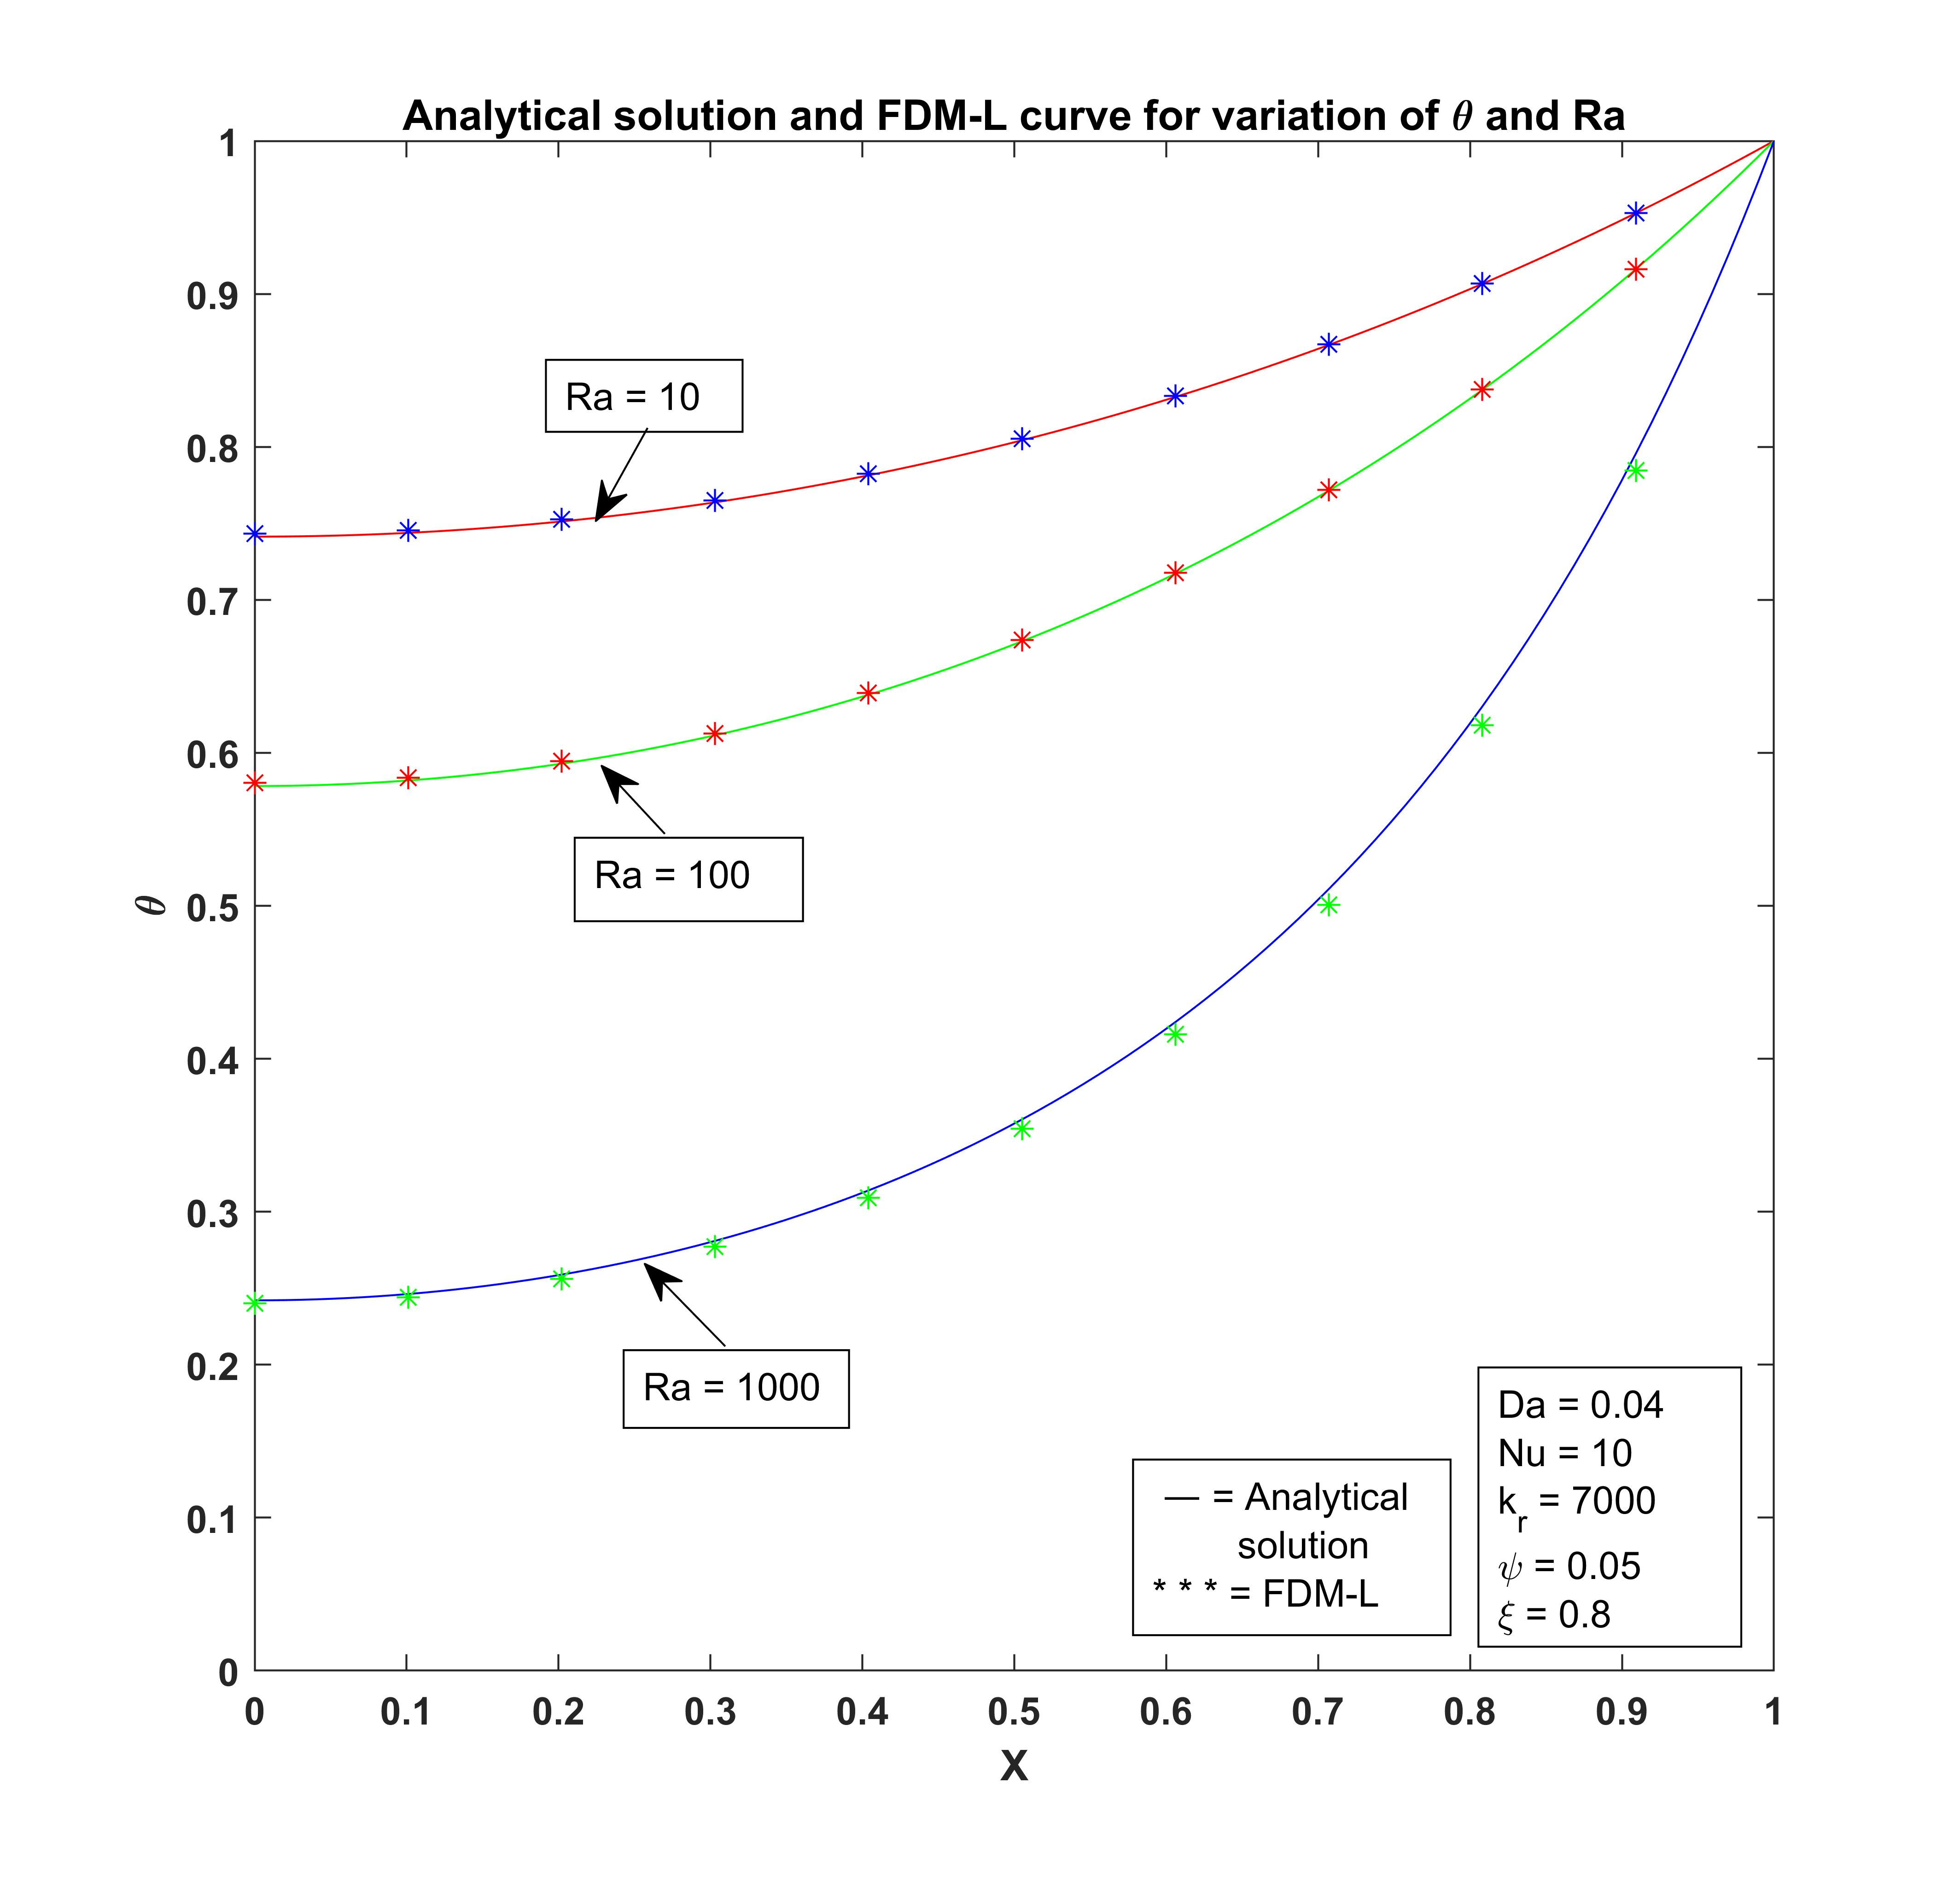
\includegraphics[scale=0.05]{Numerical Methods/LFDM/FDM L Fig3a.jpg}
  \label{fig:24}
\end{minipage}%
\begin{minipage}{.5\textwidth}
  \hspace{0.0cm}
  \vspace{-1.8cm}
  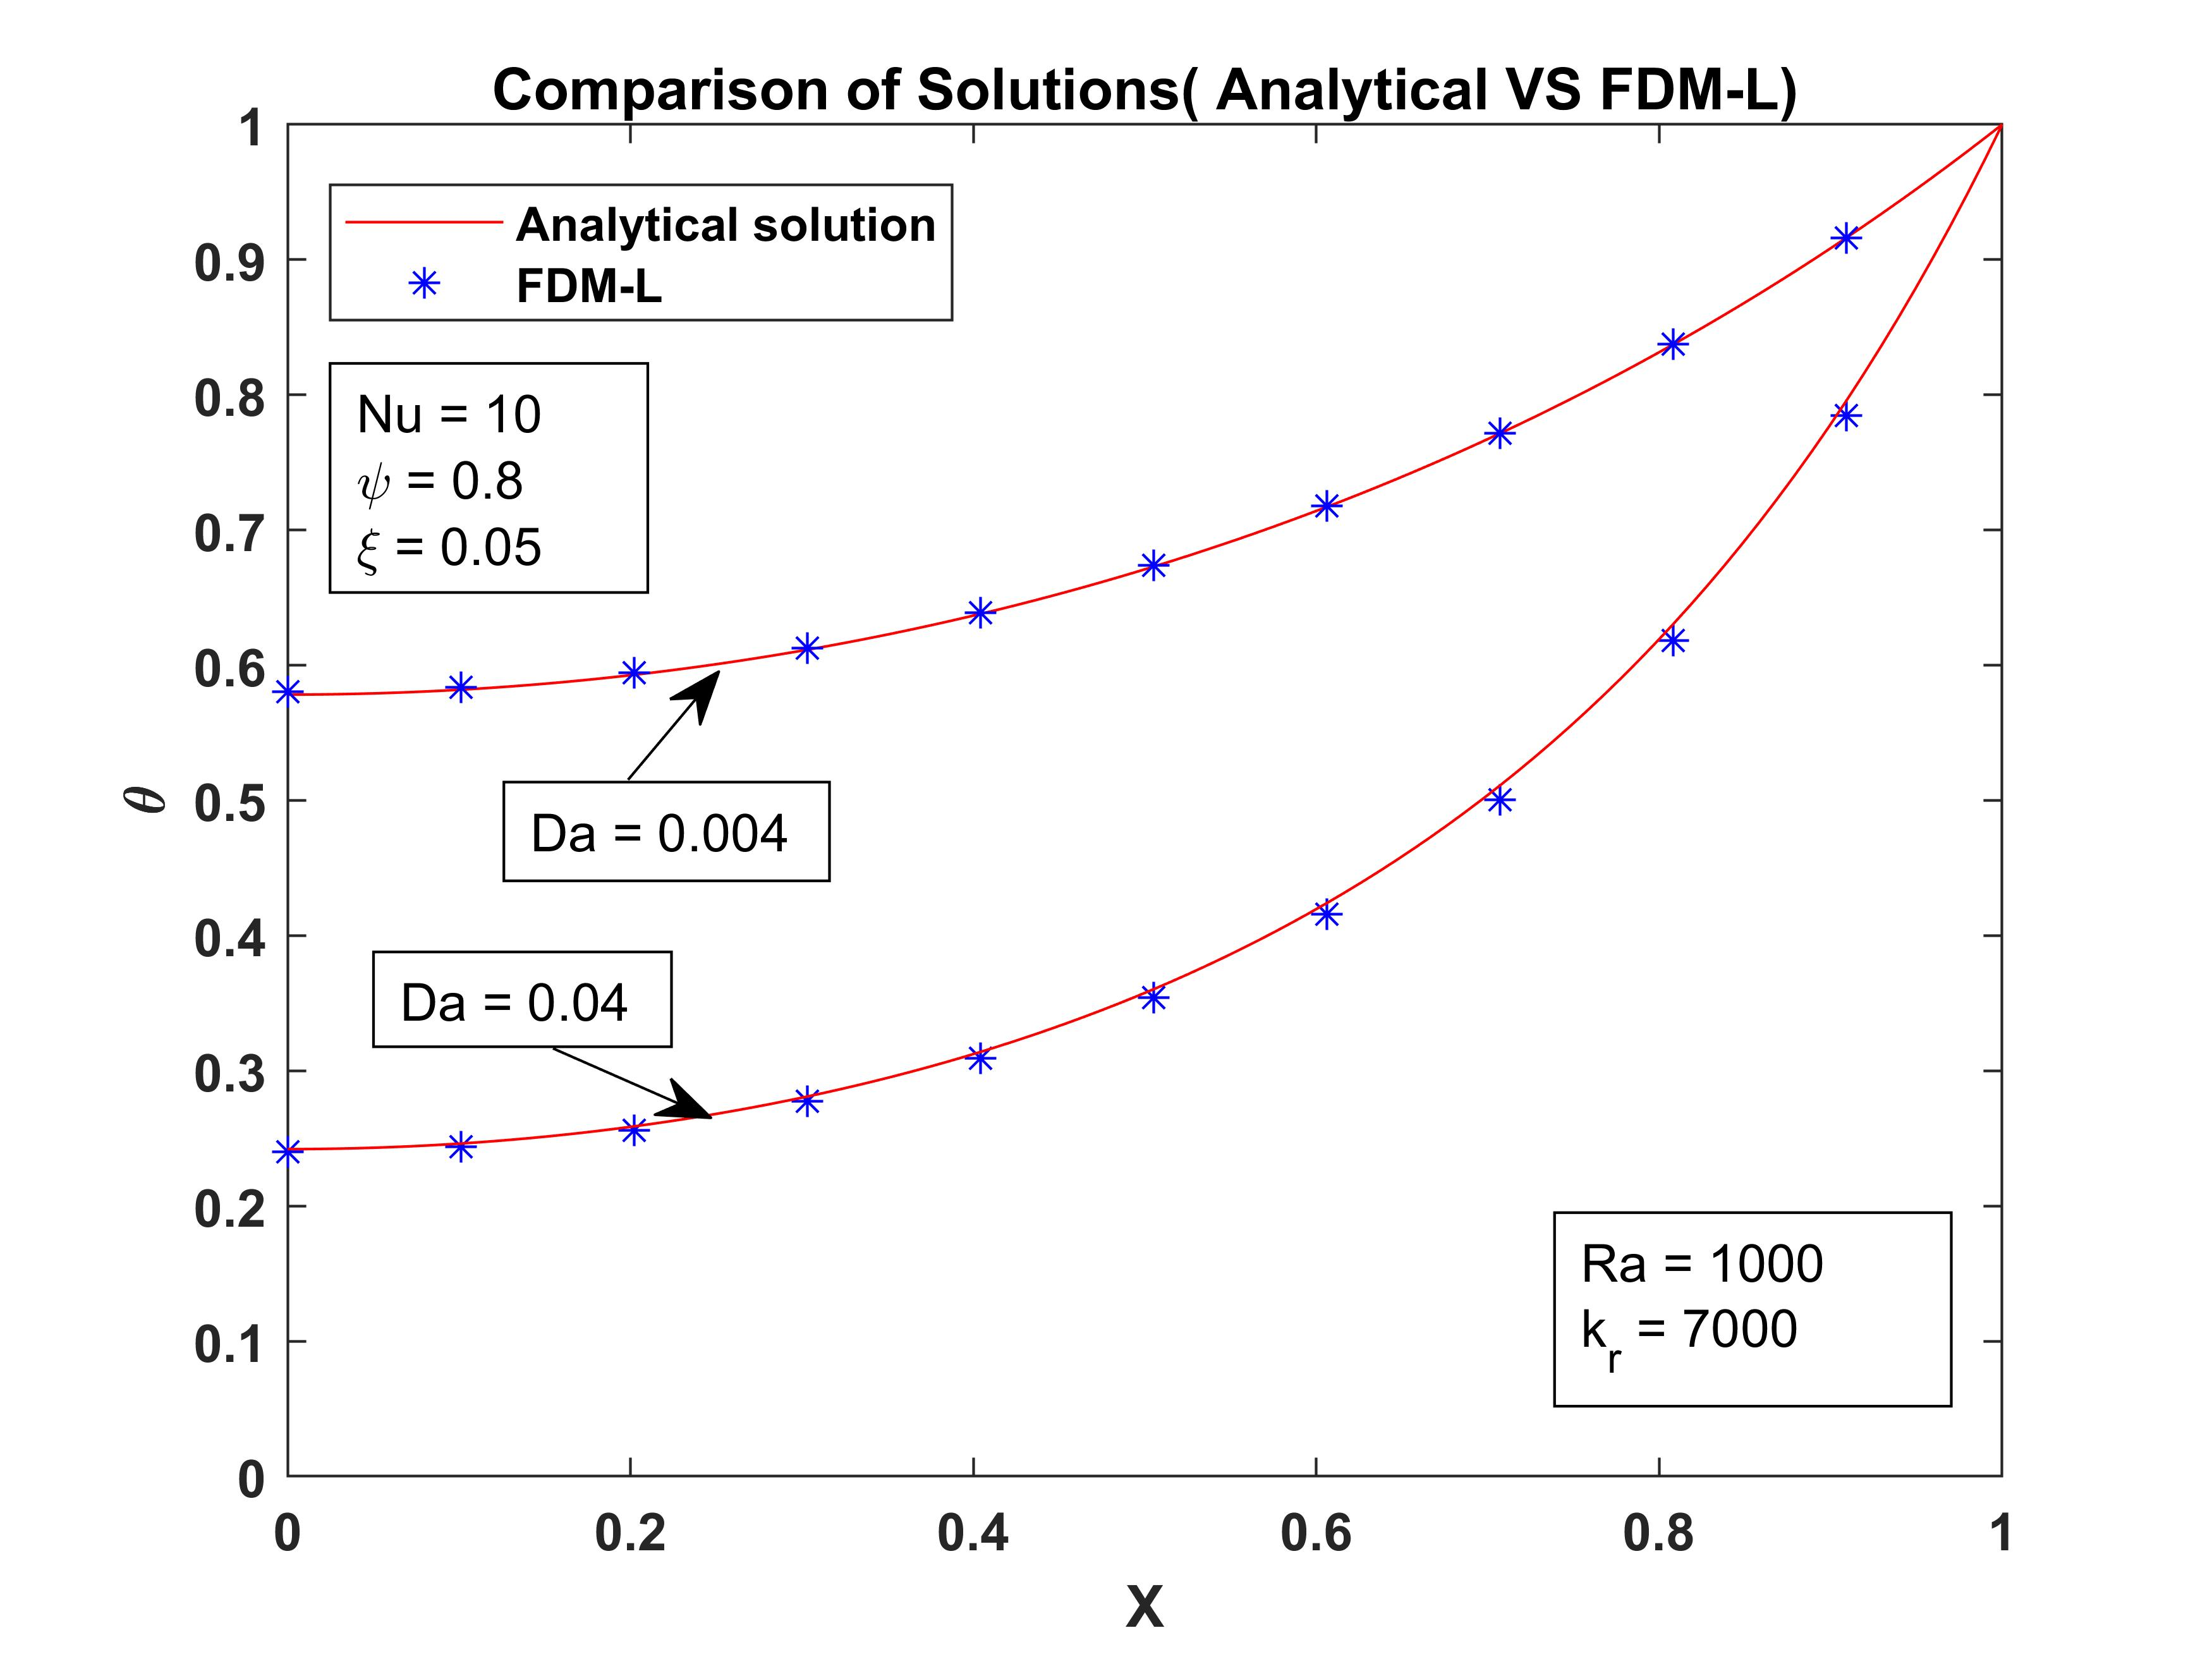
\includegraphics[scale=.07]{Numerical Methods/LFDM/FDM L.jpg}
  \label{fig:25}
\end{minipage}
\\ \\ \\
\caption{Excellent agreement between analytical and linearized FDM}
\end{figure}
The exact values of the errors obtained between analytical and linearized FDM are presented in the next section as a part of the grid independence study. It is however apparent there should be any significant deviation between the errors obtained from NL-FDM and L-FDM. This is well illustrated from the data in the \href{https://docs.google.com/spreadsheets/d/14CD9h_oIQvpSYWhHdYkxh0rk-RfhSL3lAaR-XjAy2KA/edit?usp=sharing}{Google Sheets}.
\subsubsubsection{Grid Independence study}
A similar grid-independence study outlined in the previous section was performed (using the same parameters) and the solution was found to be grid independent. We present to you the results below: 

\begin{figure}[H]
\begin{minipage}{.5\textwidth}
    \hspace{-0.5cm}
    \vspace{-1.4cm}
  \includegraphics[scale=0.5]{Numerical Methods/LFDM/Mean_error_mesh.PNG}
  \label{fig:26}
\end{minipage}%
\begin{minipage}{.5\textwidth}
  \hspace{0.0cm}
  \vspace{-1.4cm}
  \includegraphics[scale=.5]{Numerical Methods/LFDM/theta_mesh.PNG}
  \label{fig:27}
\end{minipage}
\\ \\
\caption{(left)Mean errors don't cross 0.2\% (right) $\theta(1)$ is again independent of the mesh}
\end{figure}

\begin{figure}[H]
\begin{minipage}{.5\textwidth}
    \hspace{-0.5cm}
    \vspace{-0.8cm}
  \includegraphics[scale=0.5]{Numerical Methods/LFDM/Solver_run_mesh.PNG}
  \label{fig:28}
\end{minipage}%
\begin{minipage}{.5\textwidth}
  \hspace{0.0cm}
  \vspace{-1.4cm}
  \includegraphics[scale=.5]{Numerical Methods/LFDM/total_time_mesh.PNG}
  \label{fig:29}
\end{minipage}
\\ \\
\caption{(left)Mean errors don't cross 0.2\% (right) $\theta(1)$ is again independent of the mesh}
\end{figure}

A study on the parameter $Ra$ or others was skipped due to agreement between NL-FDM and L-FDM. These are well justified due to the match between analytical and L-FDM results in Figure 13. Some results:(run time on a AMD Ryzen 5 4-core 3.6 GHz processor): 
{\begin{center}
\begin{tabularx}{0.8\textwidth} { 
  | >{\raggedright\arraybackslash}X 
  | >{\centering\arraybackslash}X 
  | >{\raggedleft\arraybackslash}X 
  | >{\raggedleft\arraybackslash}X |}
 \hline
 Mesh & Mean error[\%] & $\theta(1)$ & Run time [s] \\
 \hline
 100 & 0.1205  & 0.7433 & 0.673 \\
\hline
 200 & 0.05975 & 0.7423 & 4.791 \\
\hline
 300 & 0.039677 & 0.7421 & 16.49\\
\hline
 400 & 0.02370 & 0.7420 & 39.211\\
\hline
 1000 & 0.0117 & 0.7415 & 48.00\\
 \hline
\end{tabularx}
\end{center}
}
\subsection{Finite Volume Method}
A 1-D finite volume based discretization is presented in this section. The non-linear term is modeled as a source term and is linearized using the Picard's method.  
\subsubsection{Discretization}
\subsubsubsection{Interior cells}
\\The GDE \eqref{9} is re-written as: 
\[
\frac{d^2 \theta}{dX^2} - S(\omega_1, \omega_2, \theta) = 0 \tag{41} \label{41}
\]
Integrating \eqref{41} over finite 1-D volumes of size $\Delta x$ with unit breadth and height we obtain: \[
\int_{dV} \frac{d^2 \theta}{dX^2} dX.1.1 - \int_{dV} S(\omega_1, \omega_2, \theta_P) dX.1.1 = 0 \tag{42} \label{42}
\]
Here we assume a piece-wise constant approximation for each cell $P$ with a (constant) value $\theta_P$. Hence \eqref{42} transforms to: 
\[
\frac{d \theta}{dX}\Bigr|_e - \frac{d \theta}{dX}\Bigr|_w - S(\omega_1, \omega_2, \theta_P) \Delta X = 0 \tag{43} \label{43} 
\]
Here the small letters $e$ and $w$ represent the values of the derivatives taken at the faces of the cells. These can hence be expanded as: 
\[
\frac{\theta_E - \theta_P}{\Delta X} - \frac{\theta_P - \theta_W}{\Delta X} - S(\omega_1, \omega_2, \theta_P) \Delta X = 0 \tag{44} \label{44} 
\]
Assume for the time being that the source term $S(\omega_1, \omega_2, \theta_P)$ is decomposed and linearized as follows (following Picard's method): 
\[
S(\omega_1, \omega_2, \theta_P) = S_C(\omega_1, \omega_2, \theta_P) + S_P(\omega_1, \omega_2, \theta_P) \theta_P \tag{45} \label{45}
\]
Here $S_C$ and $S_P$ are constants that can be evaluated from the $\theta_P's$ of the previous iteration i.e.
\[
S(\omega_1, \omega_2, \theta_P^{k}) = S_C(\omega_1, \omega_2, \theta_P^{k}) + S_P(\omega_1, \omega_2, \theta_P^{k}) \theta_P^{k+1} \tag{46} \label{46}
\]
Following a simple Jacobi's method of iteration for the resulting equation system resulting from \eqref{44}, we may rewrite \eqref{44} as: 
\[
\frac{\theta_E^k - \theta_P^{k+1}}{\Delta X} - \frac{\theta_P^{k+1} - \theta_W^k}{\Delta X} - S_C(\omega_1, \omega_2, \theta_P^k) \Delta X - S_P(\omega_1, \omega_2, \theta_P^k) \theta_P^{k+1} \Delta X= 0 \tag{47} \label{47} 
\]
Collecting all the $\theta_P^{k+1}$'s to one side we get the update for a cell (not in the boundaries): 
\[
\theta_P^{k+1} = \frac{\theta_W^k+\theta_E^k -S_C(\omega_1, \omega_2,\theta_P^k) \Delta X^2}{2+S_P^k(\omega_1, \omega_2, \theta_P^k) \Delta X^2} = f(\theta_P^k,\theta_W^k, \theta_E^k,\omega_1, \omega_2) \tag{48} \label{48}
\]
We now have to take care of the source terms and the expressions for $S_C$ and $S_P$. For convenience let
\[
S^{k+1} = S(\omega_1, \omega_2, \theta_P^{k+1}) \tag{49} \label{49}
\]
Following Picard's method, we get: 
\[
S^{k+1} = S^k + \left(\frac{\partial S}{\partial \theta}\right)^k (\theta_P^{k+1} - \theta_P^k) \tag{50} \label{50}
\]
This can be rearranged as: 
\[
S^{k+1} = \left(S^k-\left(\frac{\partial S}{\partial \theta}\right)^k \theta_P^k\right) + \left(\left(\frac{\partial S}{\partial \theta}\right)^k \right) \theta_P^{k+1} = S_C^k + S_P^k \theta_p^{k+1} \tag{51} \label{51} 
\]
Hence: 
\[
S_C^k = S^k-\left(\frac{\partial S}{\partial \theta}\right)^k \theta_P^k \tag{52} \label{52}
\]
and
\[
S_P^k = \left(\frac{\partial S}{\partial \theta}\right)^k \tag{53} \label{53}
\]
Using the fact that:
\[
S(\omega_1, \omega_2, \theta) = \omega_1 \theta^2 + \omega_2 \theta \tag{54} \label{54}
\]
Along with \eqref{49} we obtain $S_C$ and $S_P$. However, only the derivative need definition and it is common to both $S_C$ and $S_P$ which follows from \eqref{54} and \eqref{49} as:
\[
\left(\frac{\partial S}{\partial \theta}\right)^k = \omega_2 + 2 \omega_1 \theta_P^k \tag{55} \label{55}
\]
Equations \eqref{48}, \eqref{49}, \eqref{52}, \eqref{53}, \eqref{54} and \eqref{55} constitute the update for a cell (not on the boundary) from the previous iteration to the next. We next derive the loop updates for the left and right boundaries keeping in mind the boundary conditions \eqref{15} and \eqref{16}. 
\subsubsubsection{Left Boundary} 
\\
Before we jump into the loop update for the left boundary let us put the index notation clear so that it is easy to locate where the boundaries are. Consider $(n+1)$ $\theta$ values with (1) and ($n+1$) denoting the boundary values. The indices (2,3,...,$n$) will denote the cell-centers of the $(n-1)$ cells as shown in Figure \ref{fig:10}. Hence, the mesh spacing and the cell size will be: $\frac{1}{n-1}$ for $n-1$ cells. Note that the value of $n$ has been chosen such that it denotes the cell-center of the last cell. We now have to take care of the first cell's discretization. The cell center is $\theta_2$ the left and right face values are $\theta_1$ and $\theta_3$ respectively. Repeating the integration from \eqref{42} and noting that the second derivative term $\frac{d\theta}{dX}\Bigr|_w$ is zero thanks to the BC \eqref{16} we get the following: 
\[
\frac{\theta_3^k -\theta_2^{k+1}}{\Delta X} = (S_{C}(\omega_1, \omega_2, \theta_2^k) + S_{P}(\omega_1, \omega_2, \theta_2^k) \theta_2^{k+1} ) \Delta X \label{56} \tag{56}
\]
Where $S_C$ and $S_P$ are already defined from \eqref{49}, \eqref{52}, \eqref{53}, \eqref{54} and \eqref{55}. We now collect all $\theta_2^{k+1}$'s to one side obtain the required loop update:
\[
\theta_2^{k+1} = \frac{\theta_3^k - S_C(\omega_1,\omega_2,\theta_2^k) \Delta X^2}{1 + S_P(\omega_1, \omega_2, \theta_2^k)} \label{57} \tag{57}
\]
\subsubsubsection{Right Boundary}
For the right boundary, the value at the right face of the last cell is fixed i.e. $\theta_{n+1} = 1$. Also while computing the derivative $\frac{d\theta}{dX}\Bigr|_e$ we need to account for the shrunk cell: 
\[
\frac{d\theta}{dX}\Bigr|_e = \frac{\theta_E^{k}-\theta_P^{k+1}}{\delta X} \tag{58} = \frac{1-\theta_P^{k+1}}{\left(\frac{\Delta X}{2}\right)}\label{58}
\]
Hence after applying the modified derivative \eqref{58} and collecting terms from \eqref{47} we get: 
\[
\theta_n^{k+1} = \frac{2 + \theta_{n-1}^k - S_C(\omega_1,\omega_2,\theta_n^k) \Delta X^2}{3 + S_P(\omega_1,\omega_2,\theta_n^k) \Delta X^2} \label{59} \tag{59}
\]
\subsubsection{Algortithm}
\begin{enumerate}
    \item Read the inputs $Ra, Da, Nu, \xi, k_r, \psi$
    \item Compute $\omega_1$ and $\omega_2$ using \eqref{7}
    \item Read mesh size and compute $h$ from \eqref{37}
    \item Declare the $\theta$ array and set $\theta(n+1)=1$
    \item Begin the outer $k$ loop and repeat 6-9 until $\epsilon<tol$
    \item from ($i=2$) until $(i<n)$ do: 
    \begin{enumerate}
        \item If $i\neq2$ or $i\neq n$ update using \eqref{48}
        \item If $i=2$ update using \eqref{57}
        \item If $i=n$ update using \eqref{59}
    \end{enumerate}
    \item if $\epsilon<tol$ exit and plot results
\end{enumerate}
\subsubsection{Implementation}
The implementation for the FVM method was a little more involved due to different updates on the boundaries and calculation of the source term. A generic master function $``Finite\_Volume\_Method"$ was created with the same input parameters as for the other functions. The dependency graph for this function is presented below: 
\begin{figure}
    \centering
    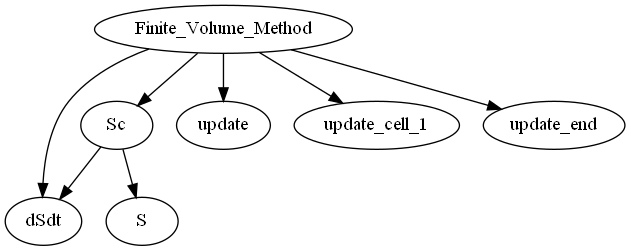
\includegraphics[scale = 0.8]{Call graphs/FVM_call_graph.png}
    \caption{Dependency graph for the master function of FVM}
    \label{fig:30}
\end{figure}
The updates and source term functions are implemented as separate dependencies to eliminate any possible coding error. The points at the FVM grid were interpolated (averaged) to the FDM grid to compare between FDM and FVM. The results of this code are presented in the next section. 
\subsubsection{Results and validation}
The results from FVM agree exactly with the previous two methods, hence confirming the solution obtained.
\begin{figure}[H]
    \centering
    \includegraphics[scale =.3]{Mesh_100_FVM.jpg}
    \caption{FVM result on 100 cell mesh}
    \label{fig:31}
\end{figure}
The solutions were found to be grid-independent indicating good convergence. The discretizations are shown to be consistent given the analytical and the FVM result match.

\begin{figure}[H]
\begin{minipage}{.5\textwidth}
    \hspace{0.0cm}
    \vspace{-1.4cm}
  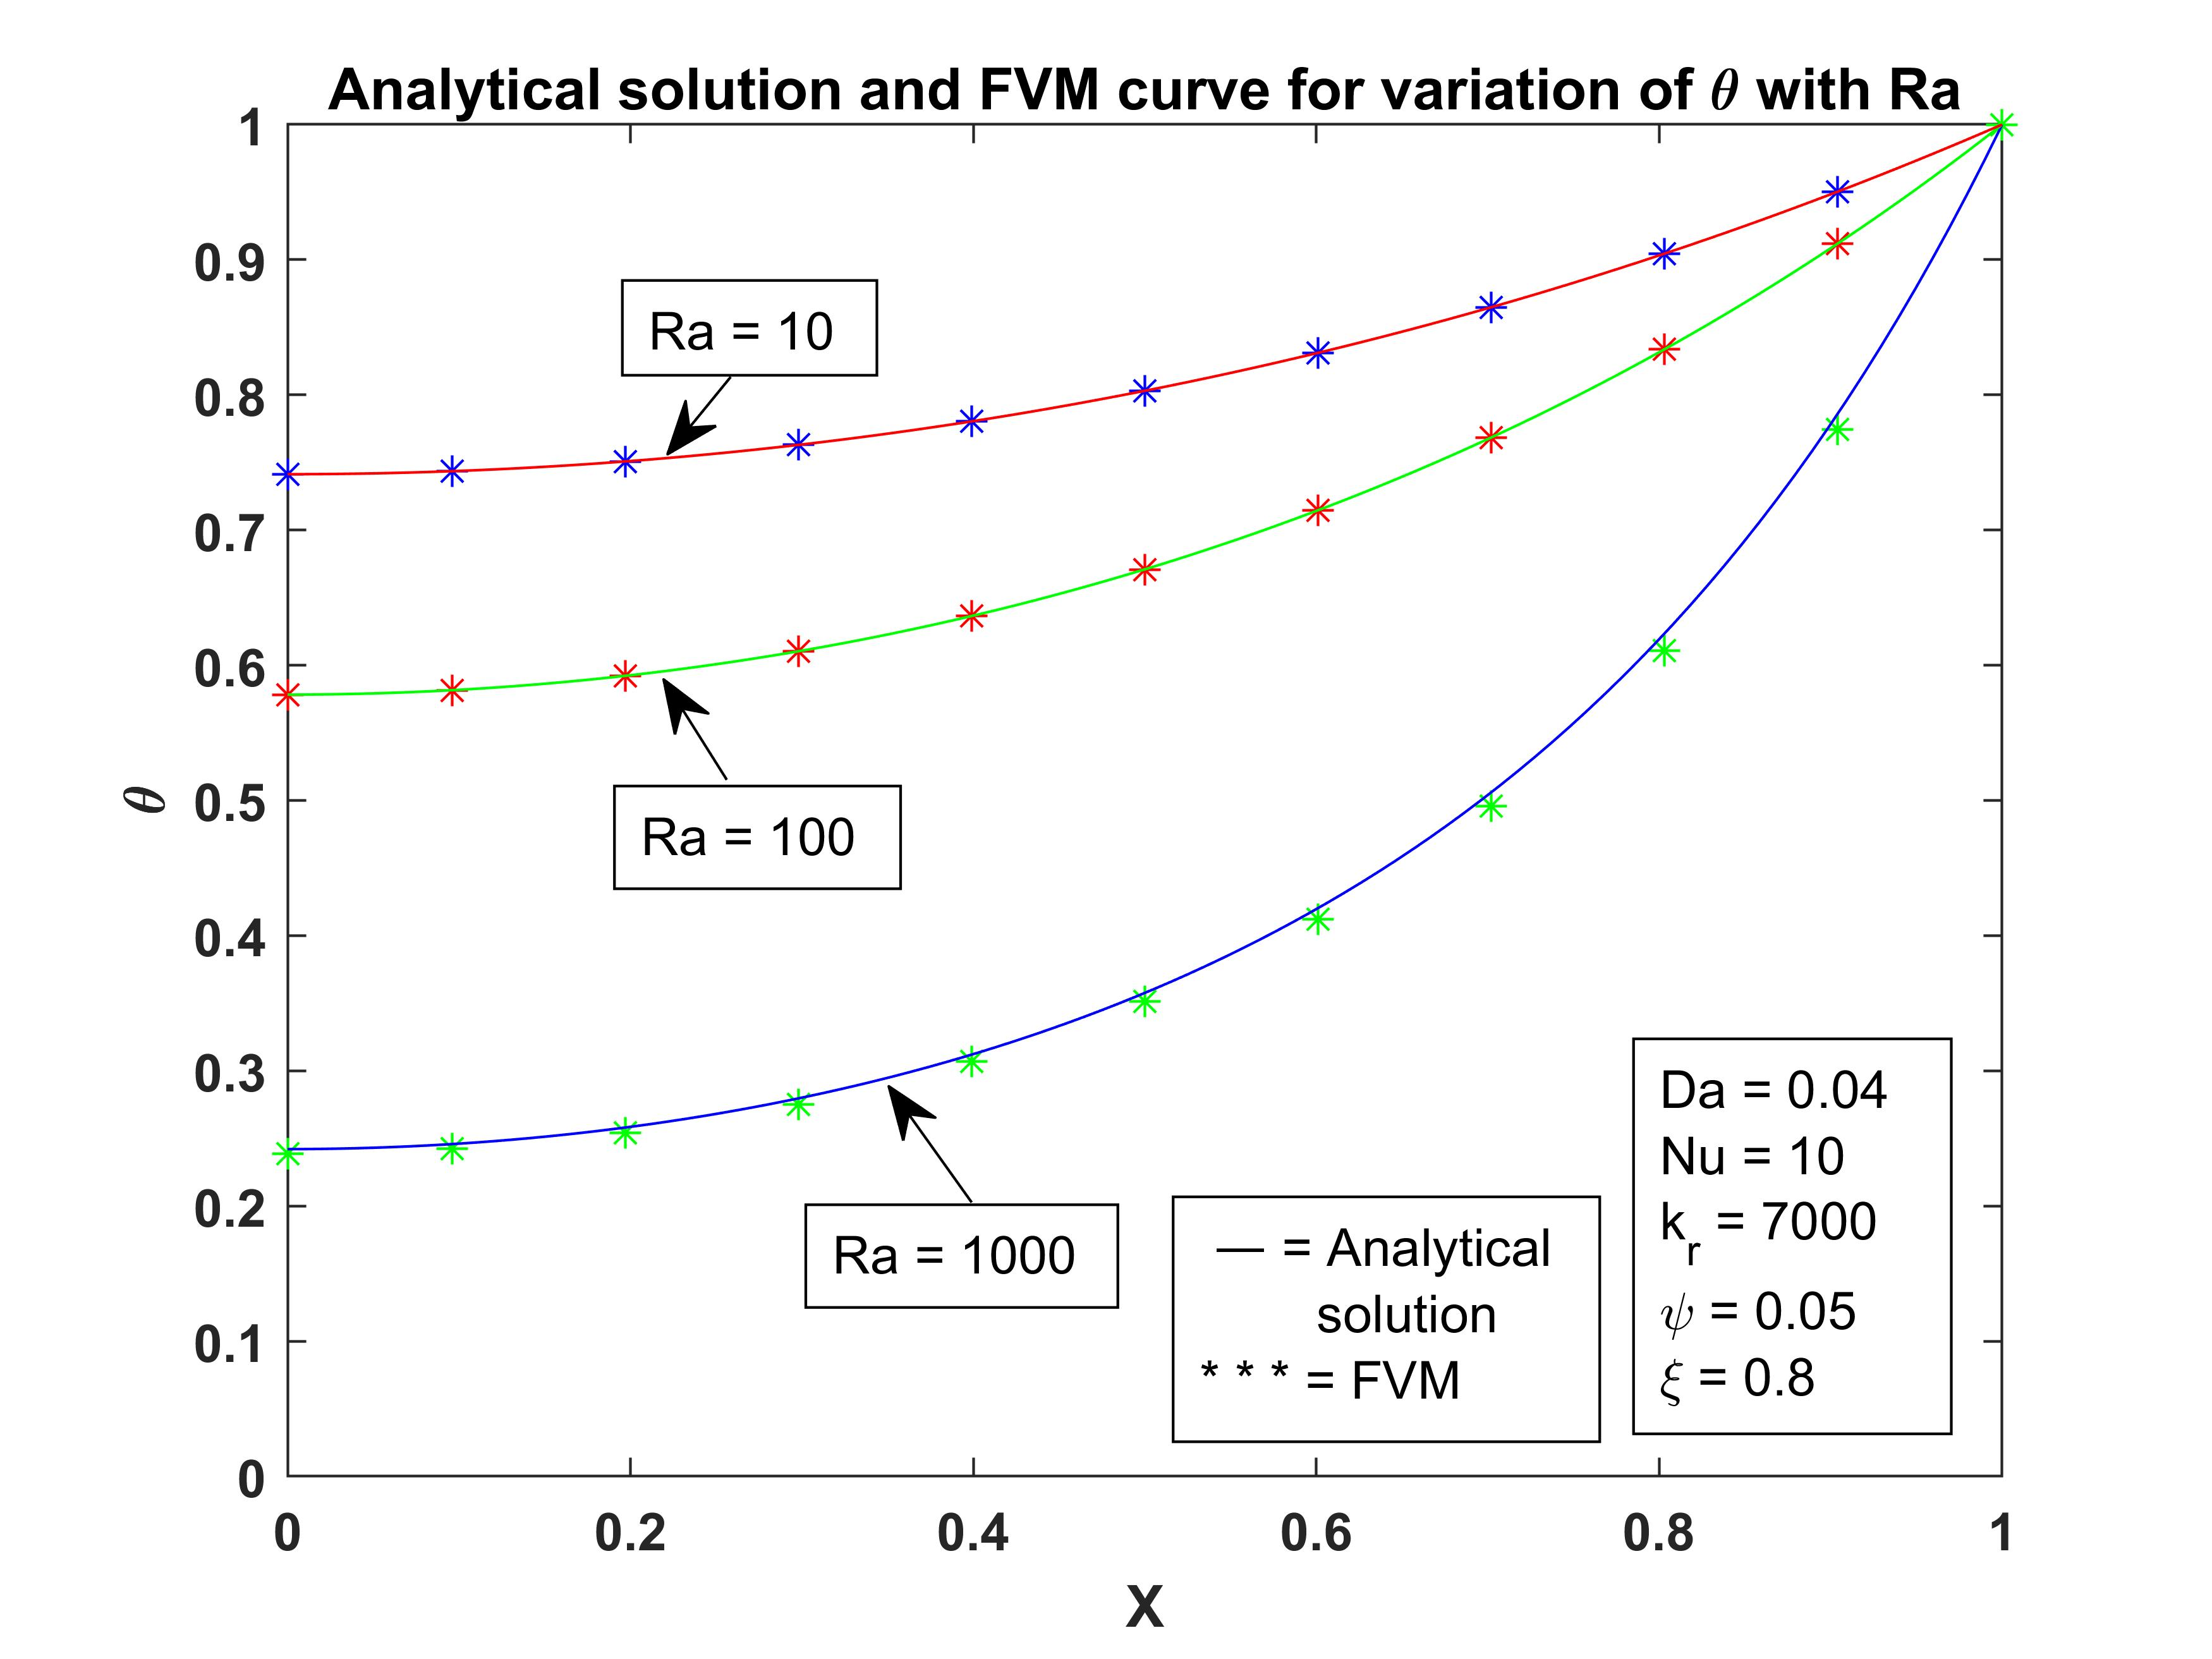
\includegraphics[scale=0.06]{Numerical Methods/FVM/FVM Fig3a.jpg}
  \label{fig:32}
\end{minipage}%
\begin{minipage}{.5\textwidth}
  \hspace{0.0cm}
  \vspace{-1.4cm}
  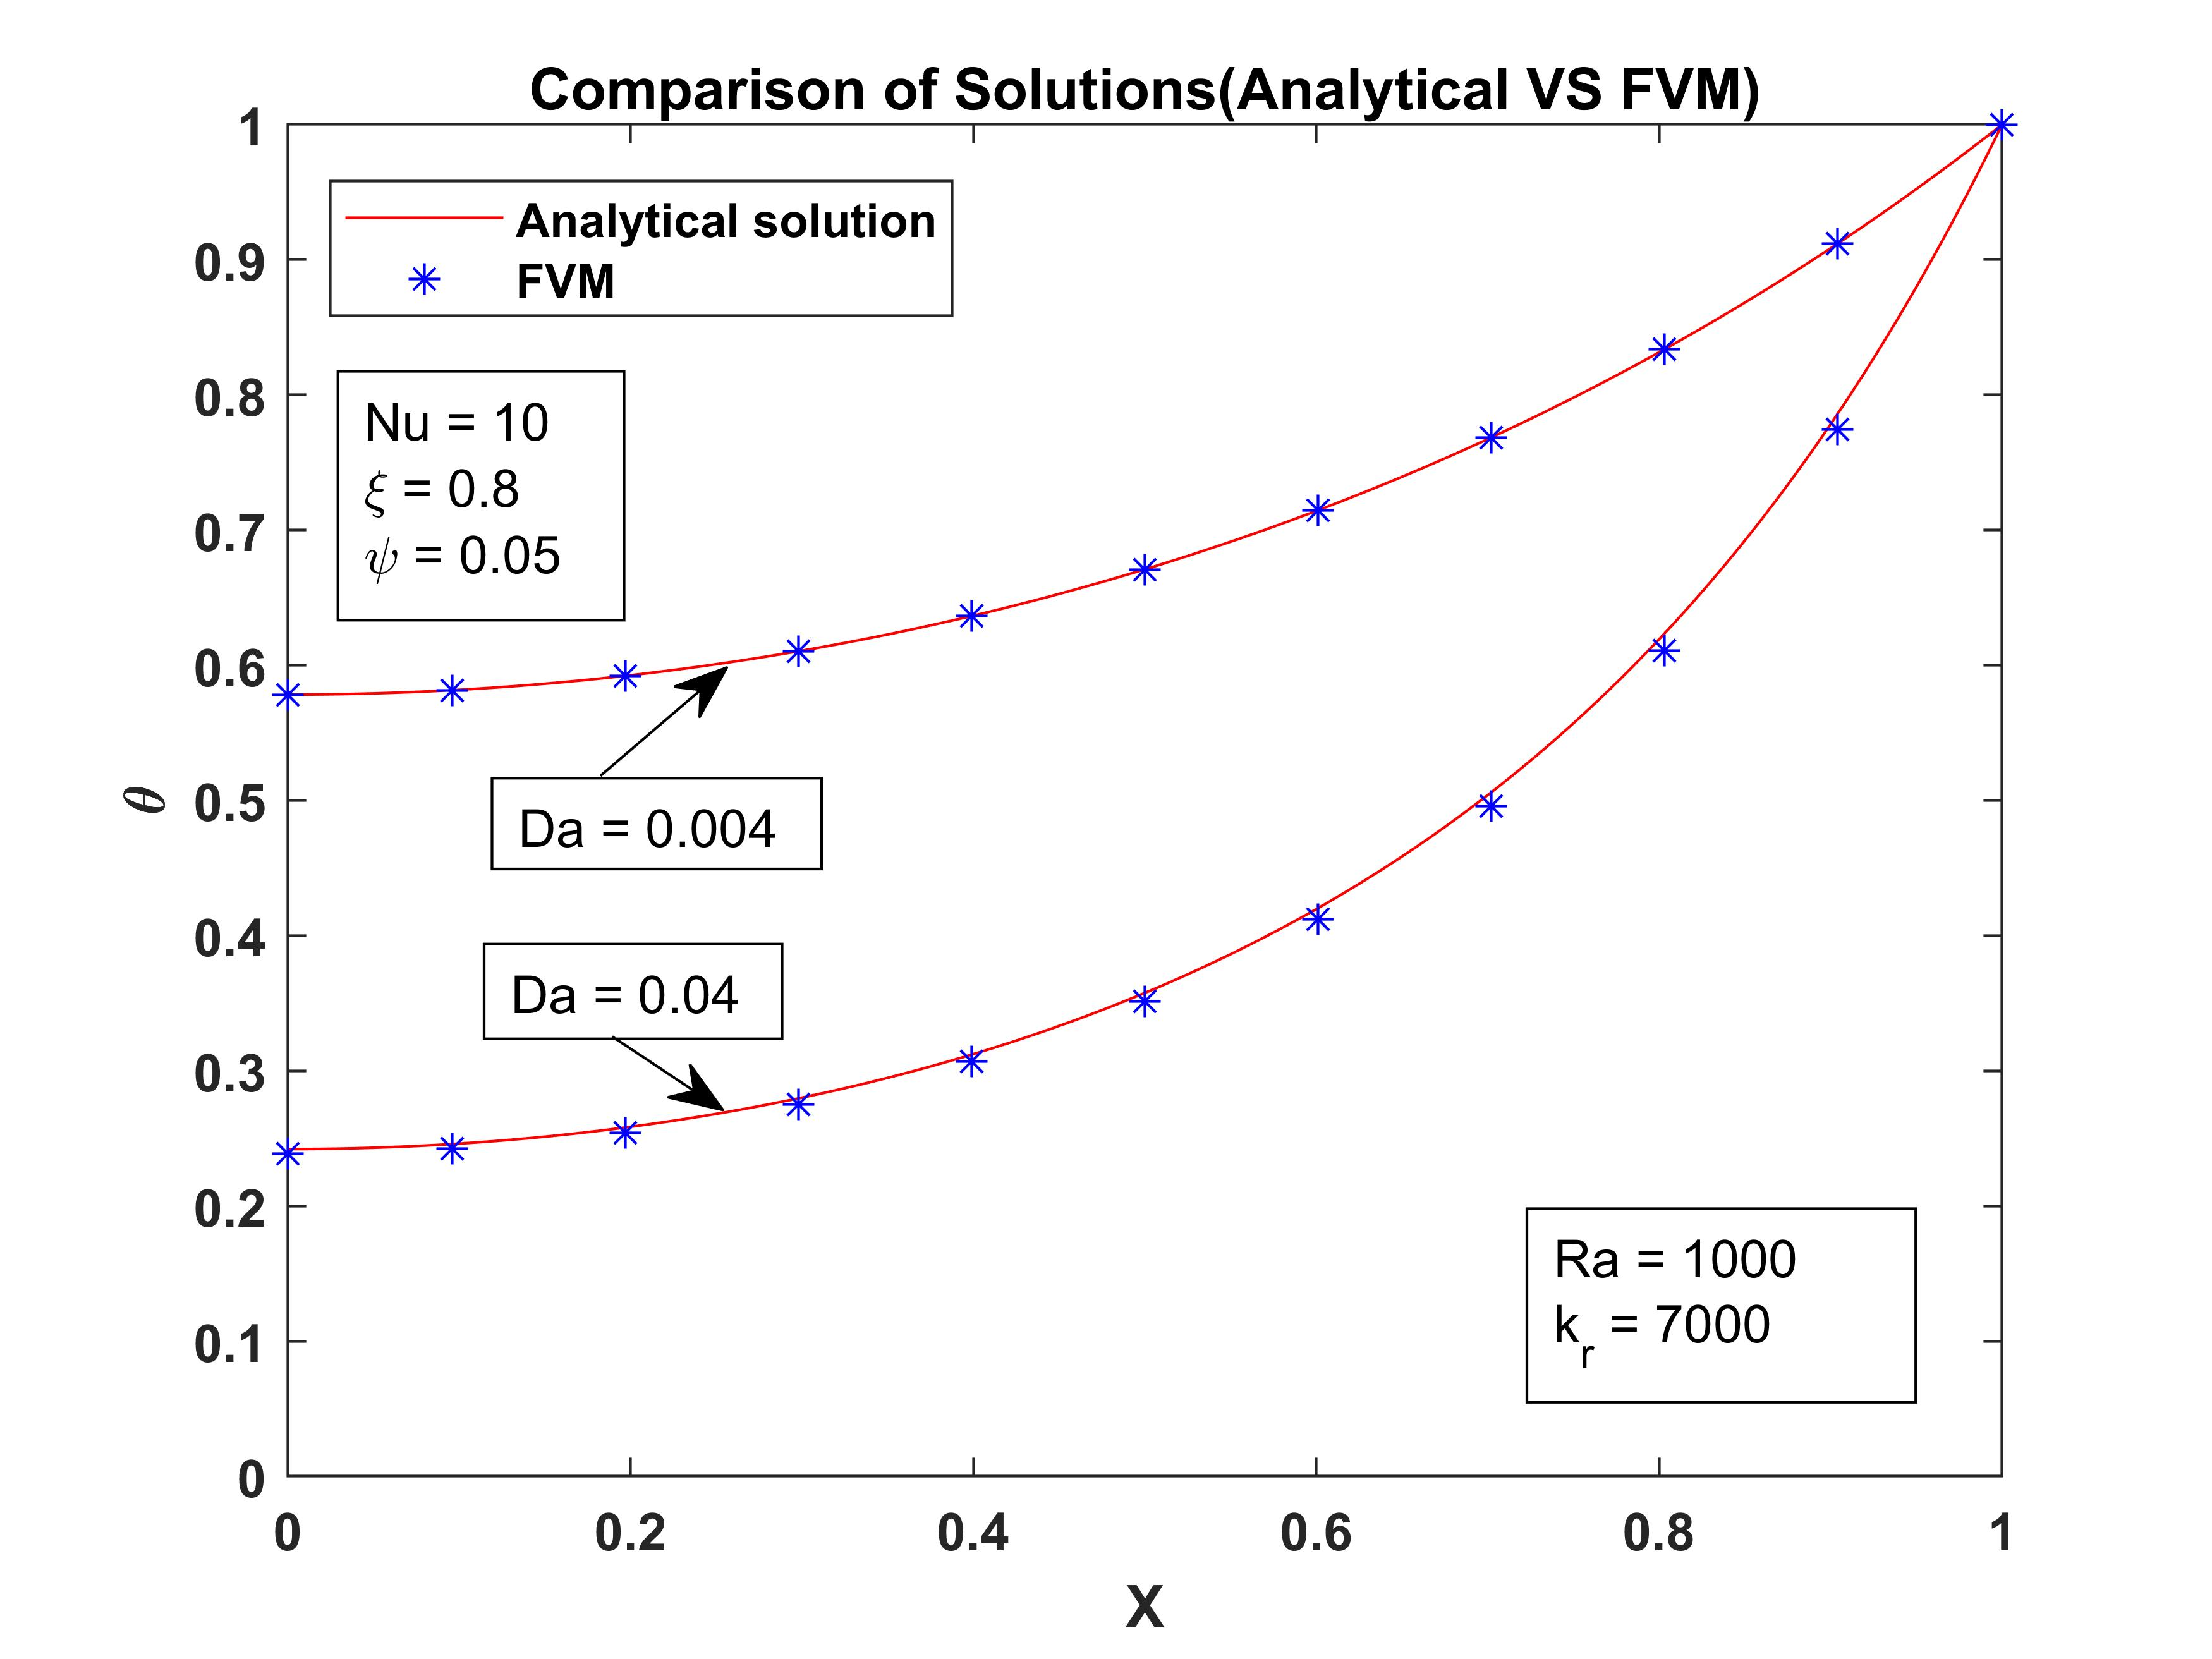
\includegraphics[scale=.06]{Numerical Methods/FVM/FVM.jpg}
  \label{fig:33}
\end{minipage}
\\ \\ \\ 
\caption{(left)Error found to decrease with mesh size (right)Identical $\theta(1)$ despite change in mesh size}
\end{figure}

\begin{figure}[H]
\begin{minipage}{.5\textwidth}
    \hspace{-1.0cm}
    \vspace{-1.0cm}
  \includegraphics[scale=0.5]{Numerical Methods/FVM/Mean_error_mesh.PNG}
  \label{fig:34}
\end{minipage}%
\begin{minipage}{.5\textwidth}
  \hspace{0.0cm}
  \vspace{-1.4cm}
  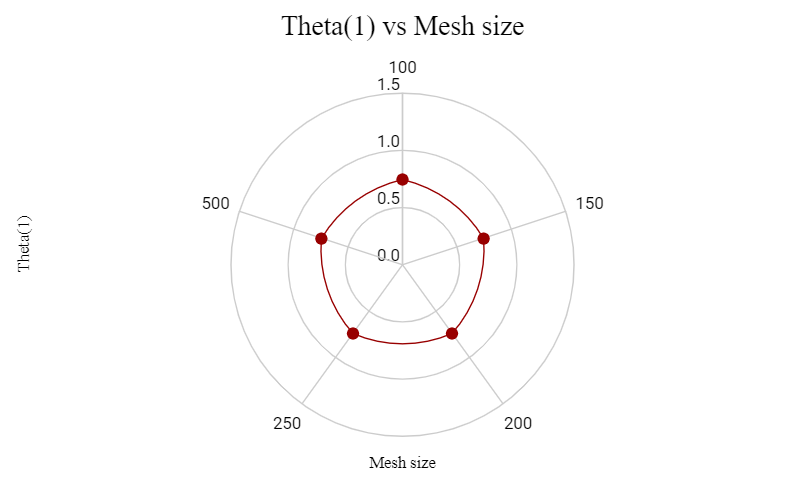
\includegraphics[scale=.5]{Numerical Methods/FVM/Theta_mesh.PNG}
  \label{fig:35}
\end{minipage}
\\ \\
\caption{(left)Error found to decrease with mesh size (right)Identical $\theta(1)$ despite change in mesh size}
\end{figure}

\begin{figure}[H]
\begin{minipage}{.5\textwidth}
    \hspace{-1.0cm}
    \vspace{-1.4cm}
  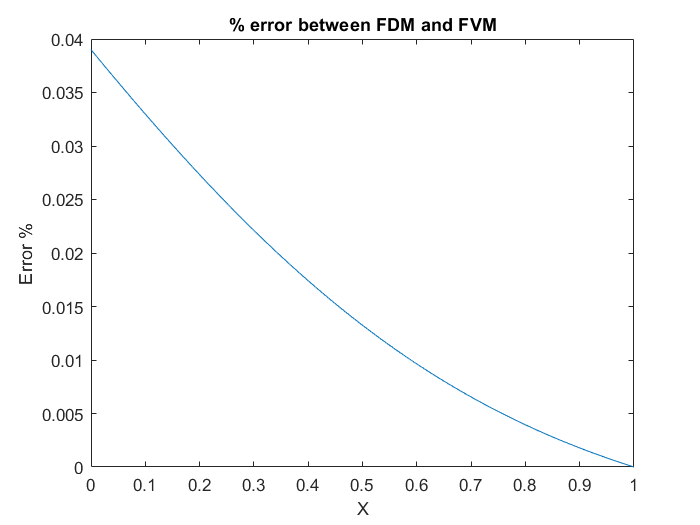
\includegraphics[scale=0.4]{error_FVM_NL.png}
  \label{fig:36}
\end{minipage}%
\begin{minipage}{.5\textwidth}
  \hspace{0.0cm}
  \vspace{-3cm}
  \includegraphics[scale=.45]{Numerical Methods/FVM/total_time_mesh.PNG}
  \label{fig:37}
\end{minipage}
\\ \\ \\ \\ 
\caption{(left)Error found to decrease with mesh size (right)Identical $\theta(1)$ despite change in mesh size}
\end{figure}
{\begin{center}
\begin{tabularx}{0.8\textwidth} { 
  | >{\raggedright\arraybackslash}X 
  | >{\centering\arraybackslash}X 
  | >{\raggedleft\arraybackslash}X 
  | >{\raggedleft\arraybackslash}X |}
 \hline
 Mesh & Mean error[\%] & $\theta(1)$ & Run time [s] \\
 \hline
 100 & 0.0726  & 0.7413 & 3.99 \\
\hline
 150 & 0.0485 & 0.7413 & 11.08 \\
\hline
 200 & 0.0365 & 0.7413 & 20.71\\
\hline
 250 & 0.0292 & 0.7413 & 37.44\\
\hline
 500 & 0.0146 & 0.7413 & 248.00\\
 \hline
\end{tabularx}
\end{center}
}
\begin{center}
    Grid independence data for FVM
\end{center}
\section{Code development, organization and usage}\label{sec:Code}
\subsection{Development}
A \href{https://bit.ly/3wOF5EJ}{GitHub Repository} for the same was maintained to enable version control.The code was developed keeping in mind that it must be user-friendly retaining some level of flexibility and generality. A common format followed for all methods was extensive segmentation of the code and creating methods as functions. Each function return a $(mesh \times 2)$ matrix with the first column containing the dimensionless temperatures $\theta$ corresponding to the second column containing the $X$ values. So all the user has to do is to call the function the three appropriate arguments. The next section discusses the dependencies of the files and their organization. 
\subsection{Organization}
The following are the various files and their functions. Documentation of the code can be found at the \href{https://rsuryanarayan.github.io/CFD_Documentation/}{M2HTML docs}. The user is advised to click on the ``Graphs" link in the documentation to view the call graphs. The source code organization hence will be clear. Source code in a more readable format is available here. The next section provides detailed steps for testing out the code.
\begin{figure}[H]
    \centering
    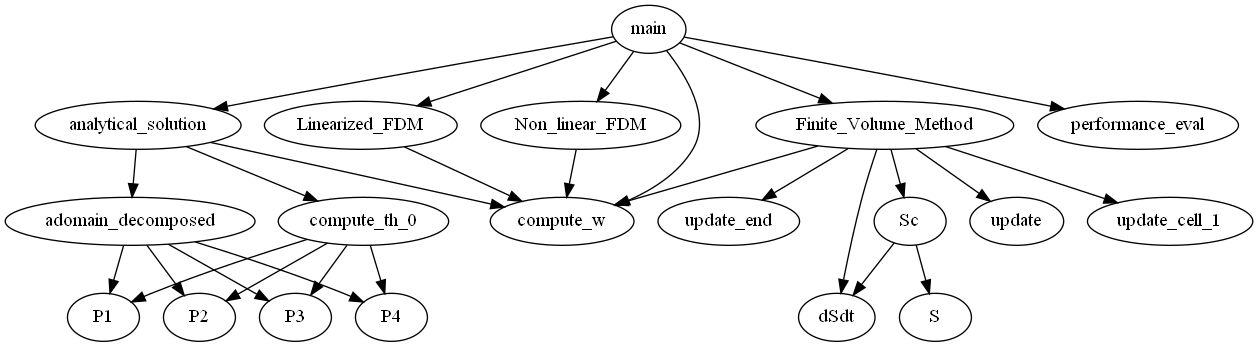
\includegraphics[scale=.4]{Call graphs/Tool_box_call_graph.png}
    \caption{The overall dependency graph of our code}
    \label{fig:38}
\end{figure}
\subsection{Usage}
The reader is referred to visit the \href{https://bit.ly/3aa4or7}{Usage.md} file of the repository that explains what one can do to run the various methods. The input argument ``params" is an array whose elements are as follows: 
\[
params = \{Ra, Da, Nu, \psi, \xi, k_r\} \tag{60} \label{60}
\]
The other two arguments are the mesh size and the tolerance for the residuals. Some quick points while running the code are:
\begin{itemize}
    \item Download the entire  \href{https://github.com/RSuryaNarayan/CFD_MEPE11}{CFD\_MEPE11} repository. (I created another sub-folder here itself for convenience instead of a new repository, so bear with me!)
    \item Navigate to the ``Group Assignment/Code/Source"
    \item You can now either upload all of the files to MATLAB or run them on your local if you have it installed
    \item Please make sure to have all files in the same place (instead of having subfolders). For instance, cut and paste ``Source/FVM" files to ``Source/". The organization was done in github to generate suitable documentation).
    \item If you run into any issues please message Surya.
\end{itemize}
We hope that you were able to run the code smoothly! 
\clearpage
\section{Summary, Conclusion and Suggestions}
\begin{enumerate}
    \item The paper by Bhanja et.al (Procedia Engineering 64 ( 2013 ) 956 – 965) on the thermal analysis of porous pin fin used for electronic cooling was validated using suitable numerical techniques.
    \item A total of 3 numerical methods namely Non-linear Finite Difference Method, linearized Finite Difference Method and Finite Volume Method were implemented using the MATLAB programming language.
    \item The entire project was hosted on \href{https://bit.ly/3gPOgPN}{GitHub} for better collaboration. \href{https://rsuryanarayan.github.io/CFD_Documentation/}{Suitable documentation} for the code was generated to enable better understanding for users using \href{https://www.artefact.tk/software/matlab/m2html/}{M2HTML} software.
    \item Results from the numerical methods thus implemented show excellent agreement between themselves (error $\approx10^{-7}$) as well as the analytical results (error$\approx10^{-4}$).
    \item To further validate and check the accuracy of the numerical results, we performed a grid-independence study by systematically increasing the mesh size from a base of 100 to 1000.
    \item The solutions improved in accuracy with mesh refinement initially but attained constancy eventually. The time taken to compute the solutions were approximately the same however all of them exponentially increased with time.
    \item However, it is observed that small errors (of magnitudes about 0.05\% (order $\approx10^{-5}$) persist even with very fine meshes($\approx1000$).
    \item We believe that this is because of the following: \\
    (a) the approximation in the analytical solution (where its computed as a combination of adomain polynomials.The greater the number of these polynomials the better the accuracy) \\
    (b) Discretization errors in the numerical method, interpolation errors (between FDM and FVM grids)\\
    (c) Trivial coding errors, human errors etc 
\end{enumerate}
\begin{center}
    \emph{THANK YOU!}
\end{center}
%\hspace{1 cm}--- Linus
%\newpage
%\bibliographystyle{apalike}
%\bibliography{biblist}

\end{document}
